%%
%% Meta: TI nSpire Einführung
%%       Ziel: Damit die Grundoperationen damit durchgeführt werden können.
%%             Damit man sich an den Rechner gewöhnt.
%%

\input{bbwLayoutPage}

%%%%%%%%%%%%%%%%%%%%%%%%%%%%%%%%%%%%%%%%%%%%%%%%%%%%%%%%%%%%%%%%%%

\usepackage{amssymb} %% für \blacktriangleright
\renewcommand{\metaHeaderLine}{Arbeitsblatt}
\renewcommand{\arbeitsblattTitel}{Uebungen am Einheitskreis}

\begin{document}%%
\arbeitsblattHeader{}

\noTRAINER{
\begin{tabular}{ccc}
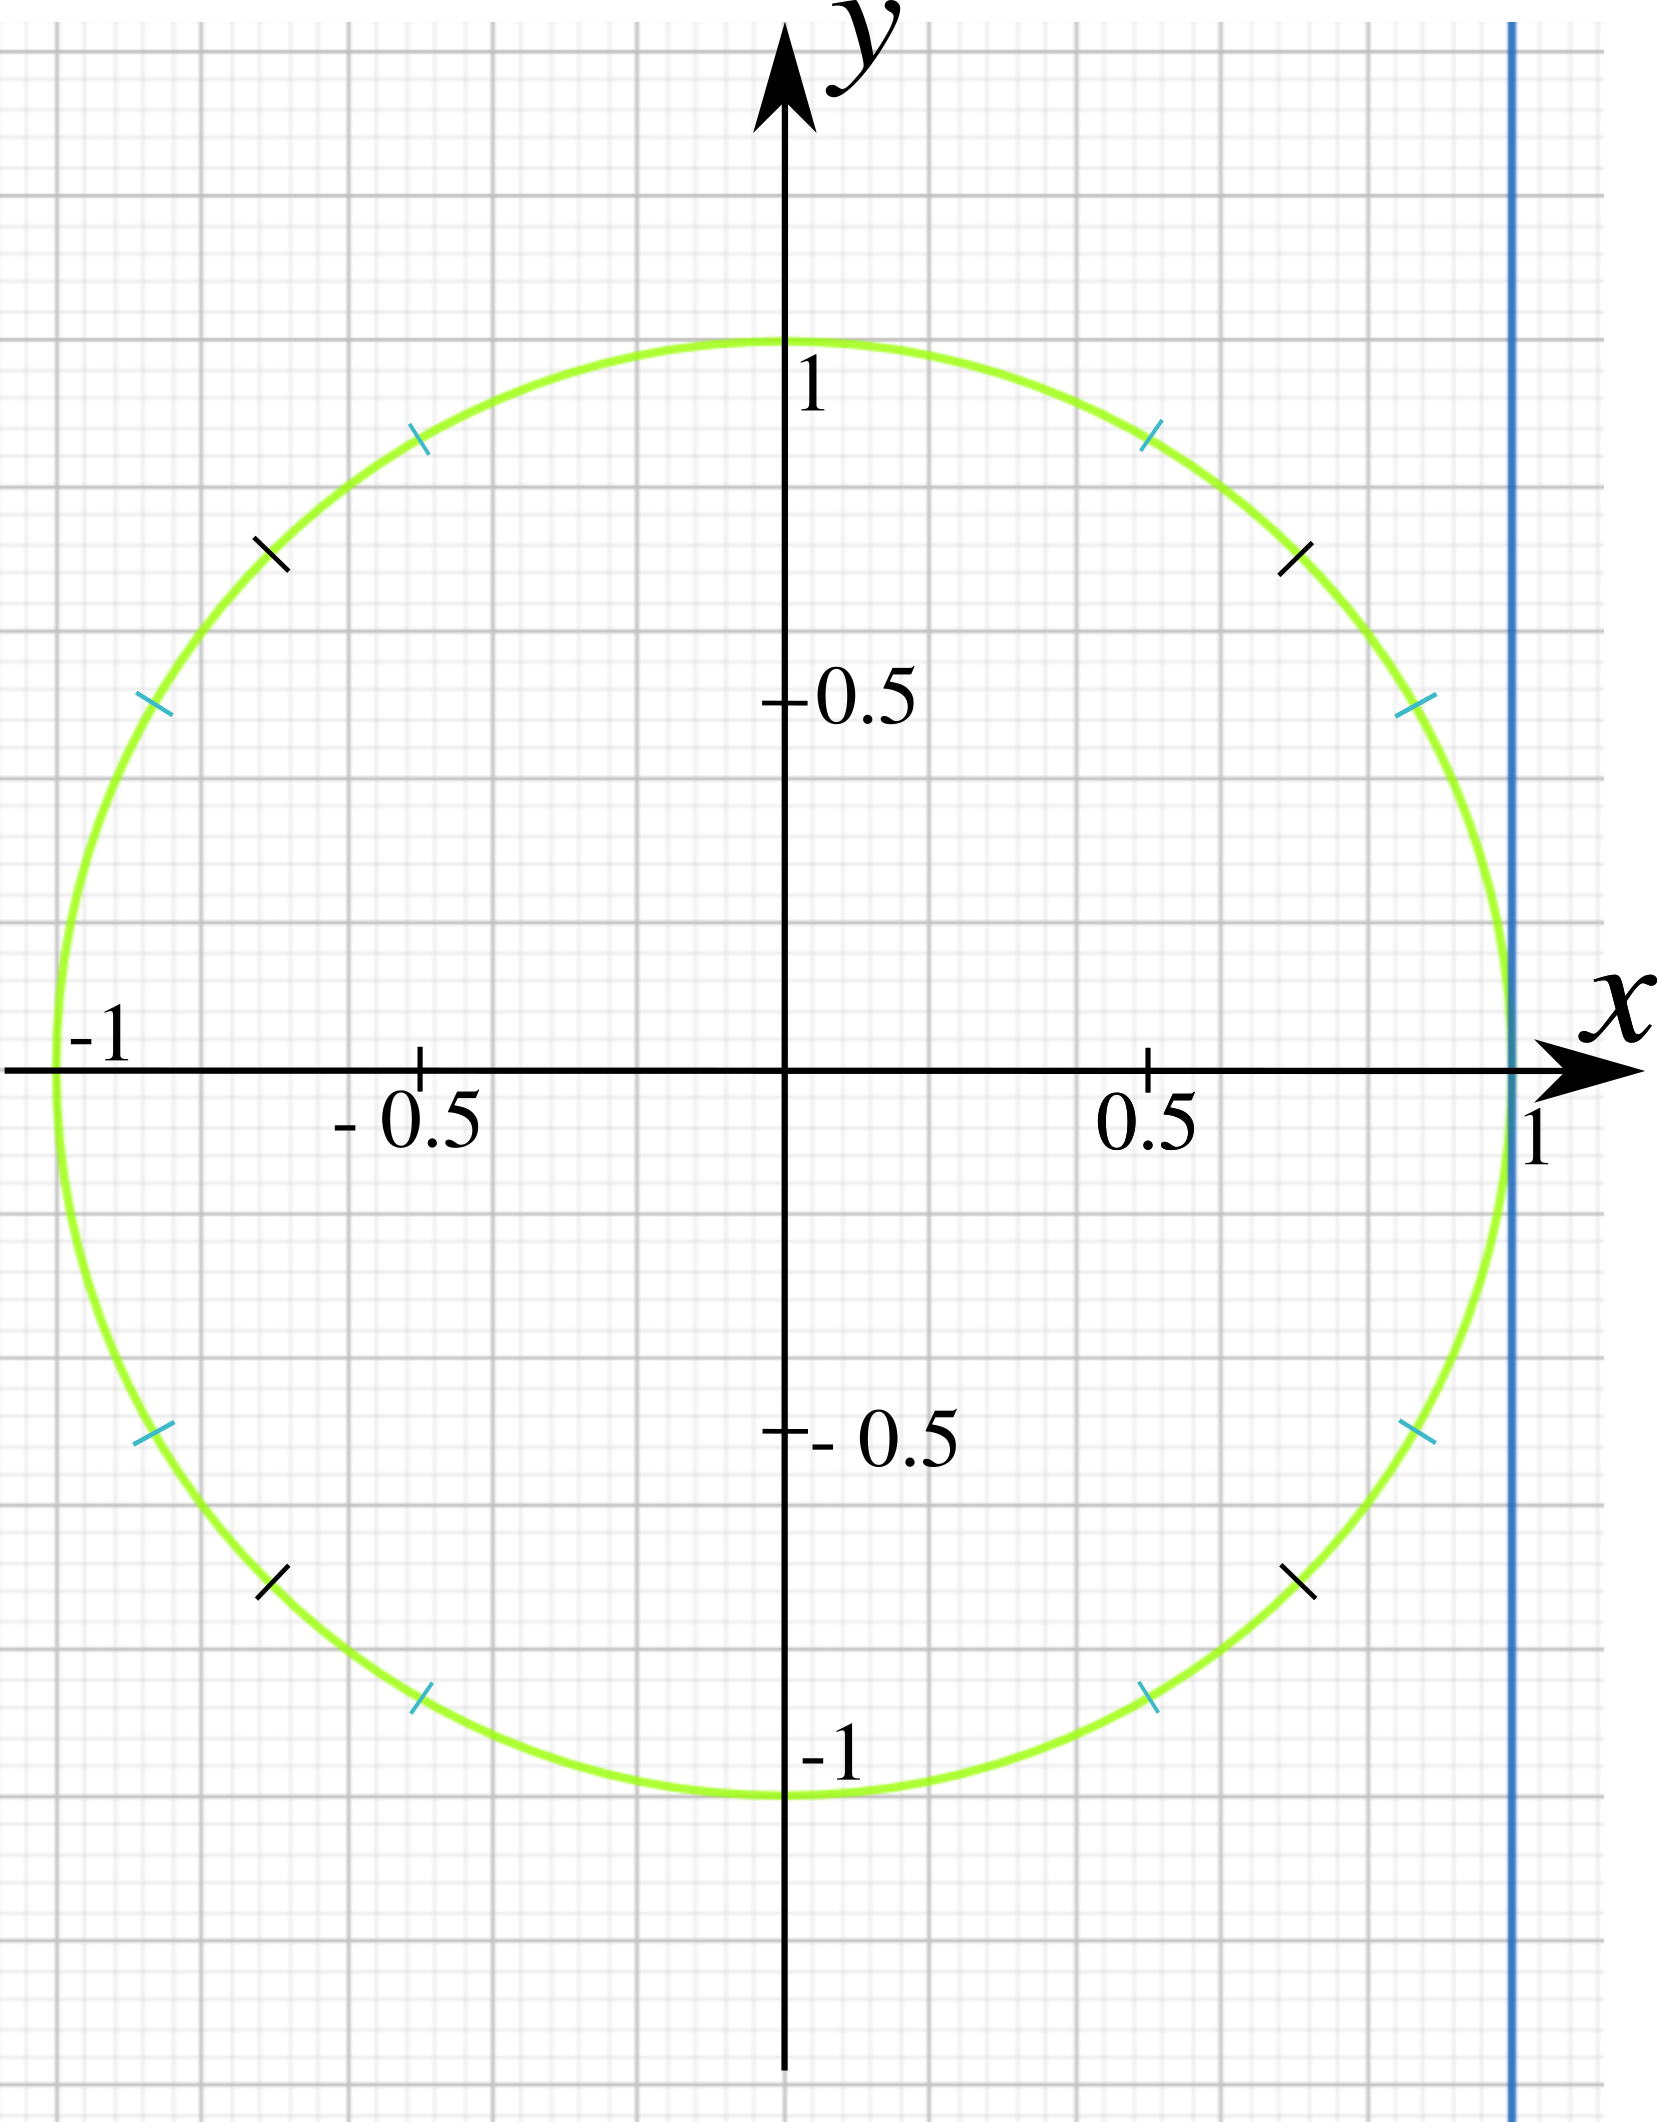
\includegraphics[width=5cm]{img/Einheitskreis304560.png} &\,\,\,\,\,\,\,\,\,\,\,\,\,\,\,\,\,\,\,\, &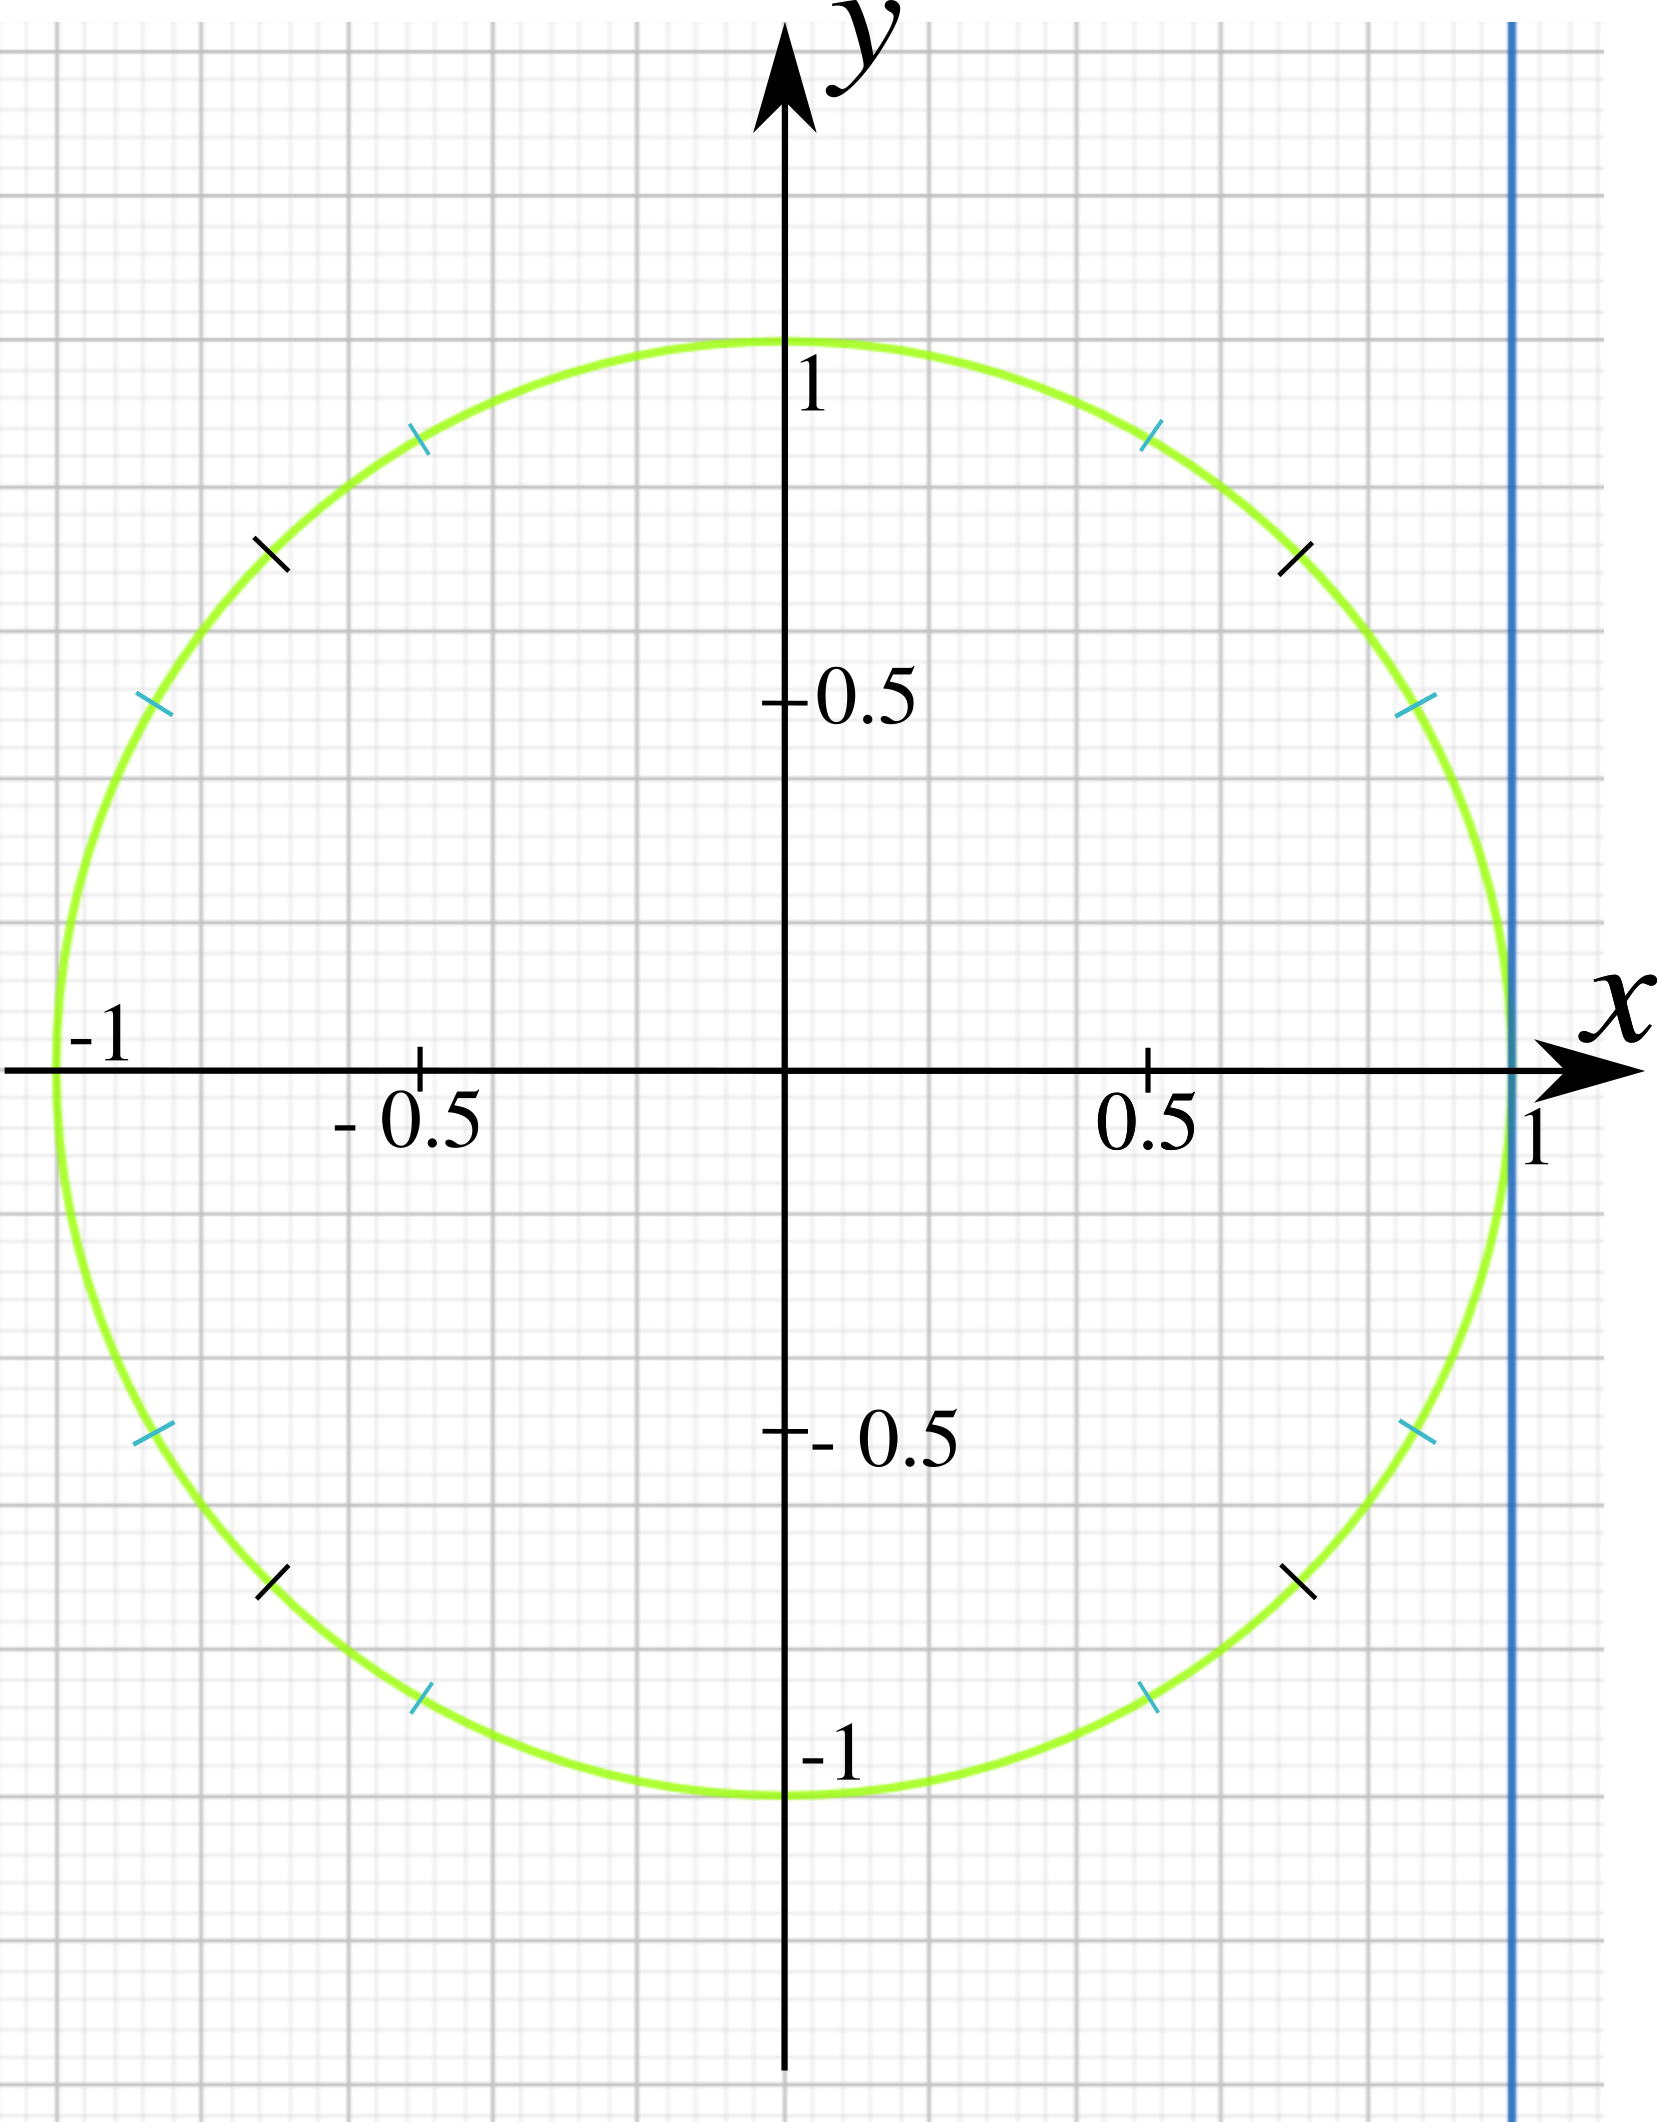
\includegraphics[width=5cm]{img/Einheitskreis304560.png}\\
\end{tabular}
}
\TRAINER{\bbwCenterGraphic{6cm}{img/Einheitskreis304560.png}}


\textbf{1. Wahr oder falsch?} (Ohne Taschenrechner)


a) $\sin(40\degre)<\tan(40\degre)$ \LoesungsRaum{Wahr}

b) $\sin(-40\degre)<\tan(140\degre)$ \LoesungsRaum{Falsch: sin(-40) = -0.62 und tan(140) = -0.84}

\noTRAINER{
\begin{tabular}{ccc}
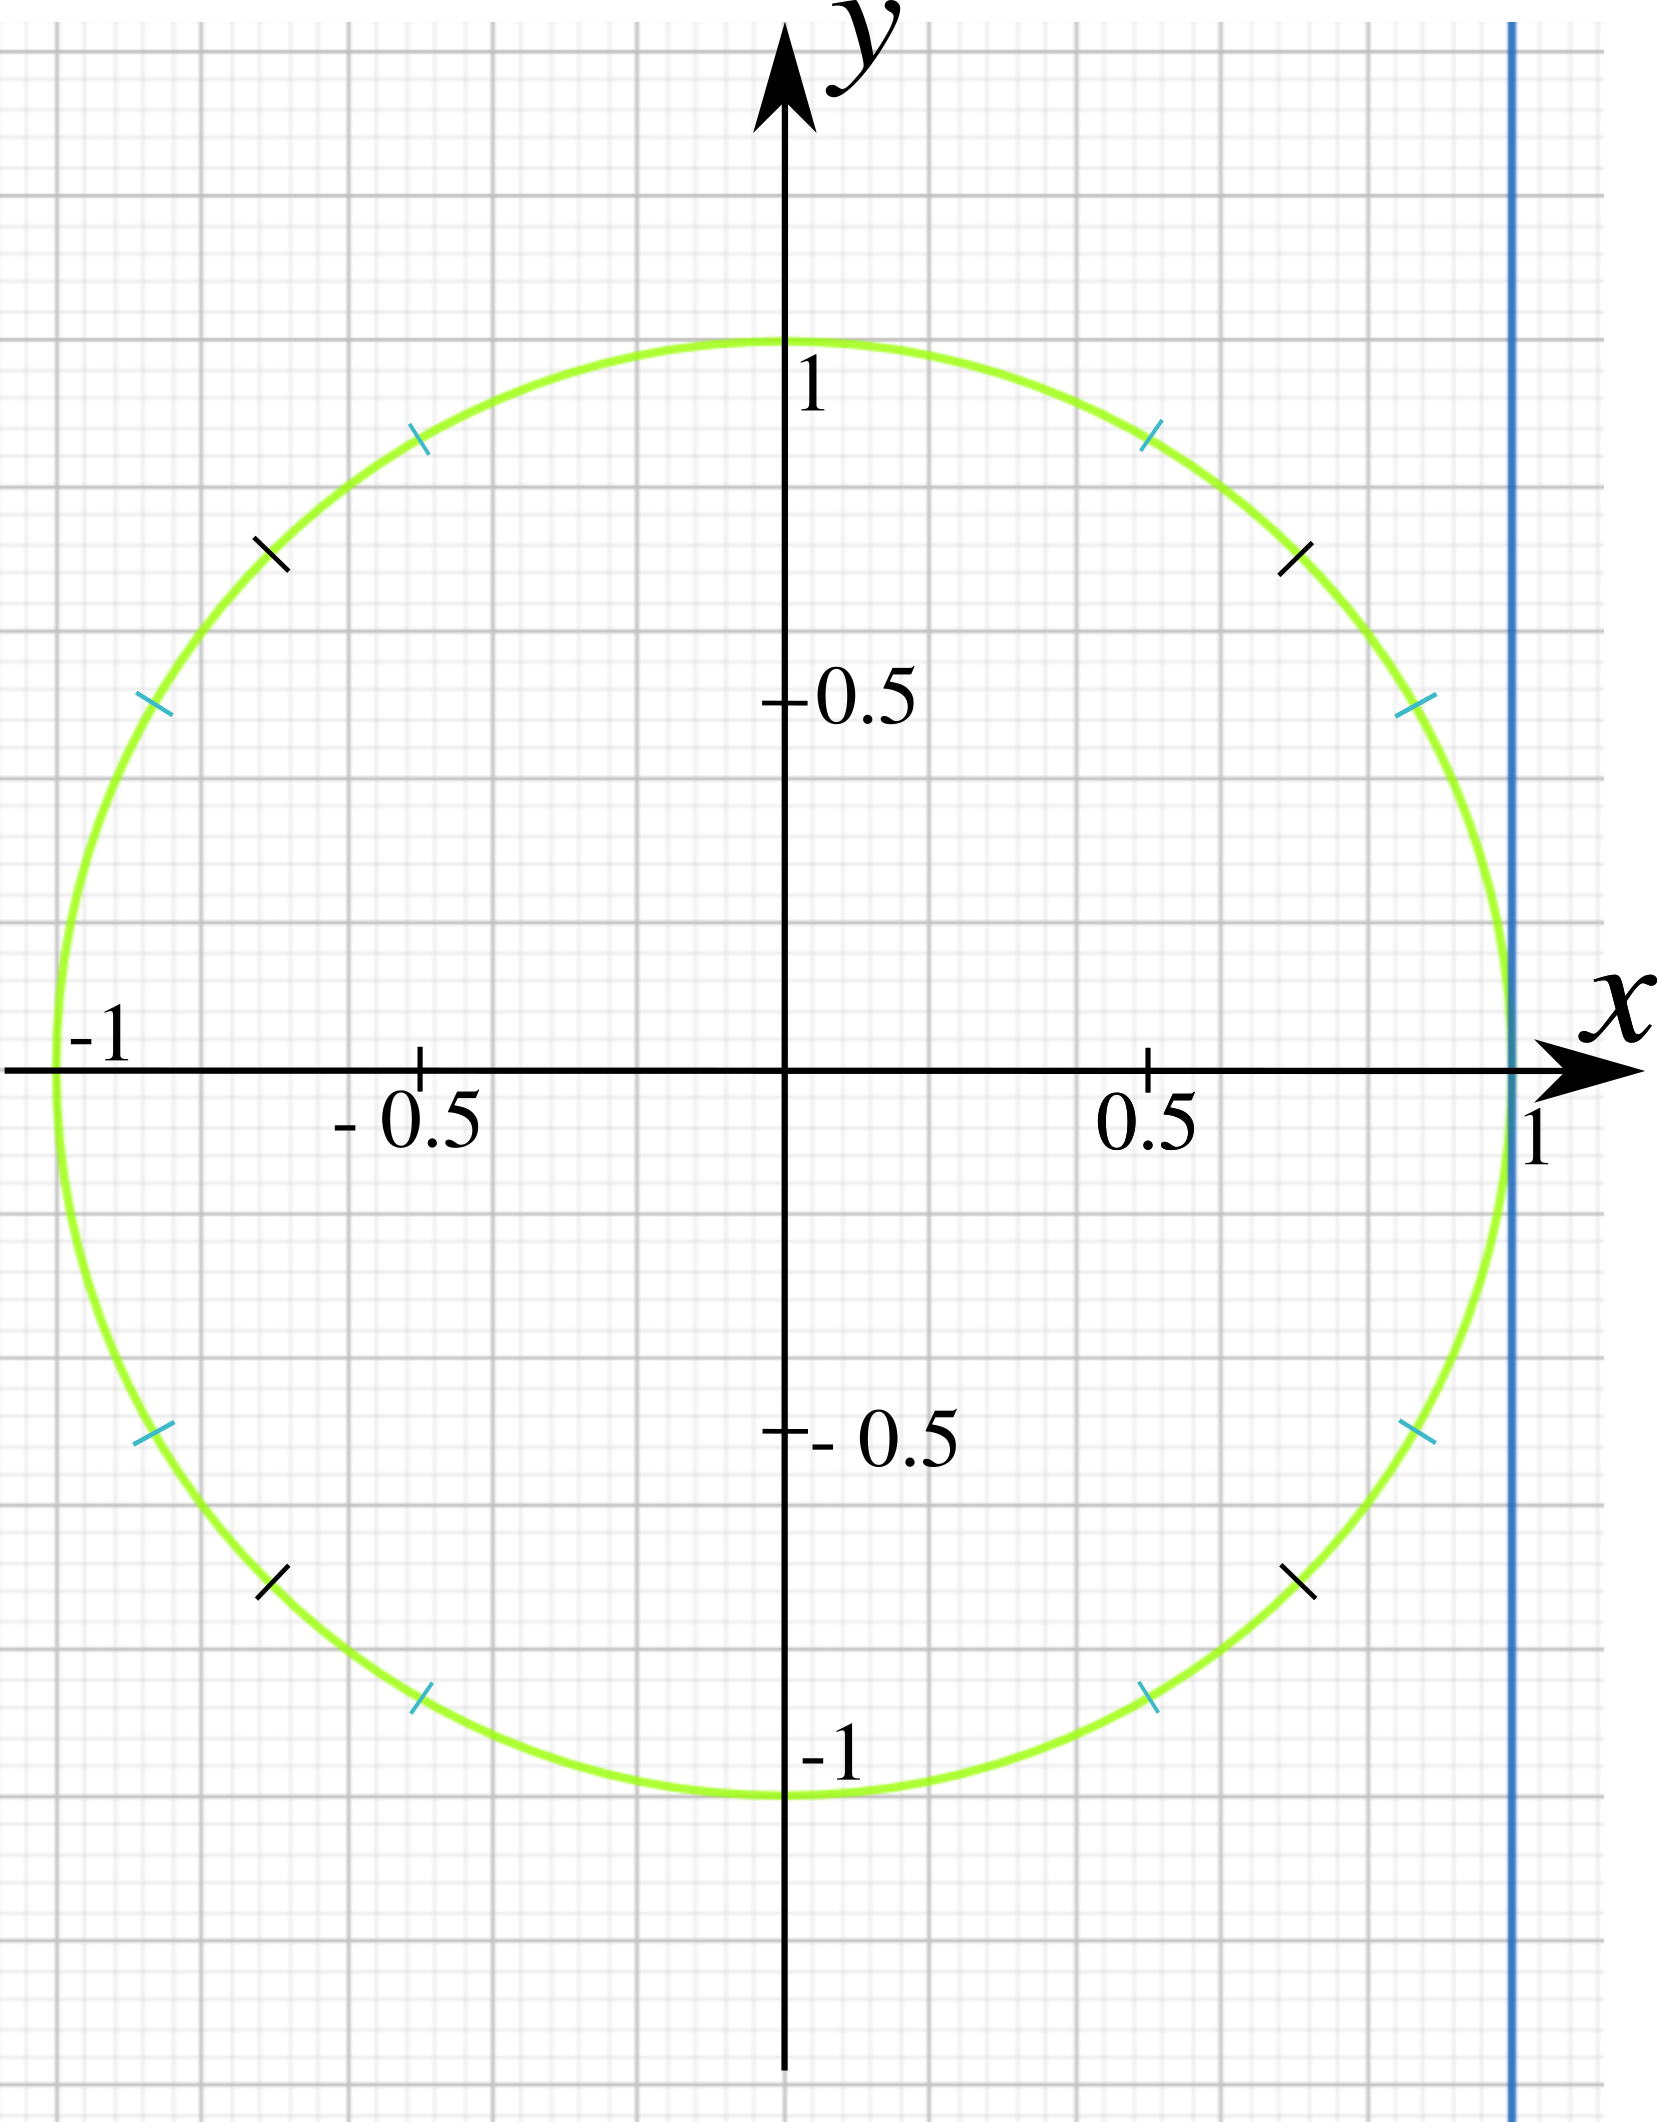
\includegraphics[width=5cm]{img/Einheitskreis304560.png} &\,\,\,\,\,\,\,\,\,\,\,\,\,\,\,\,\,\,\,\, &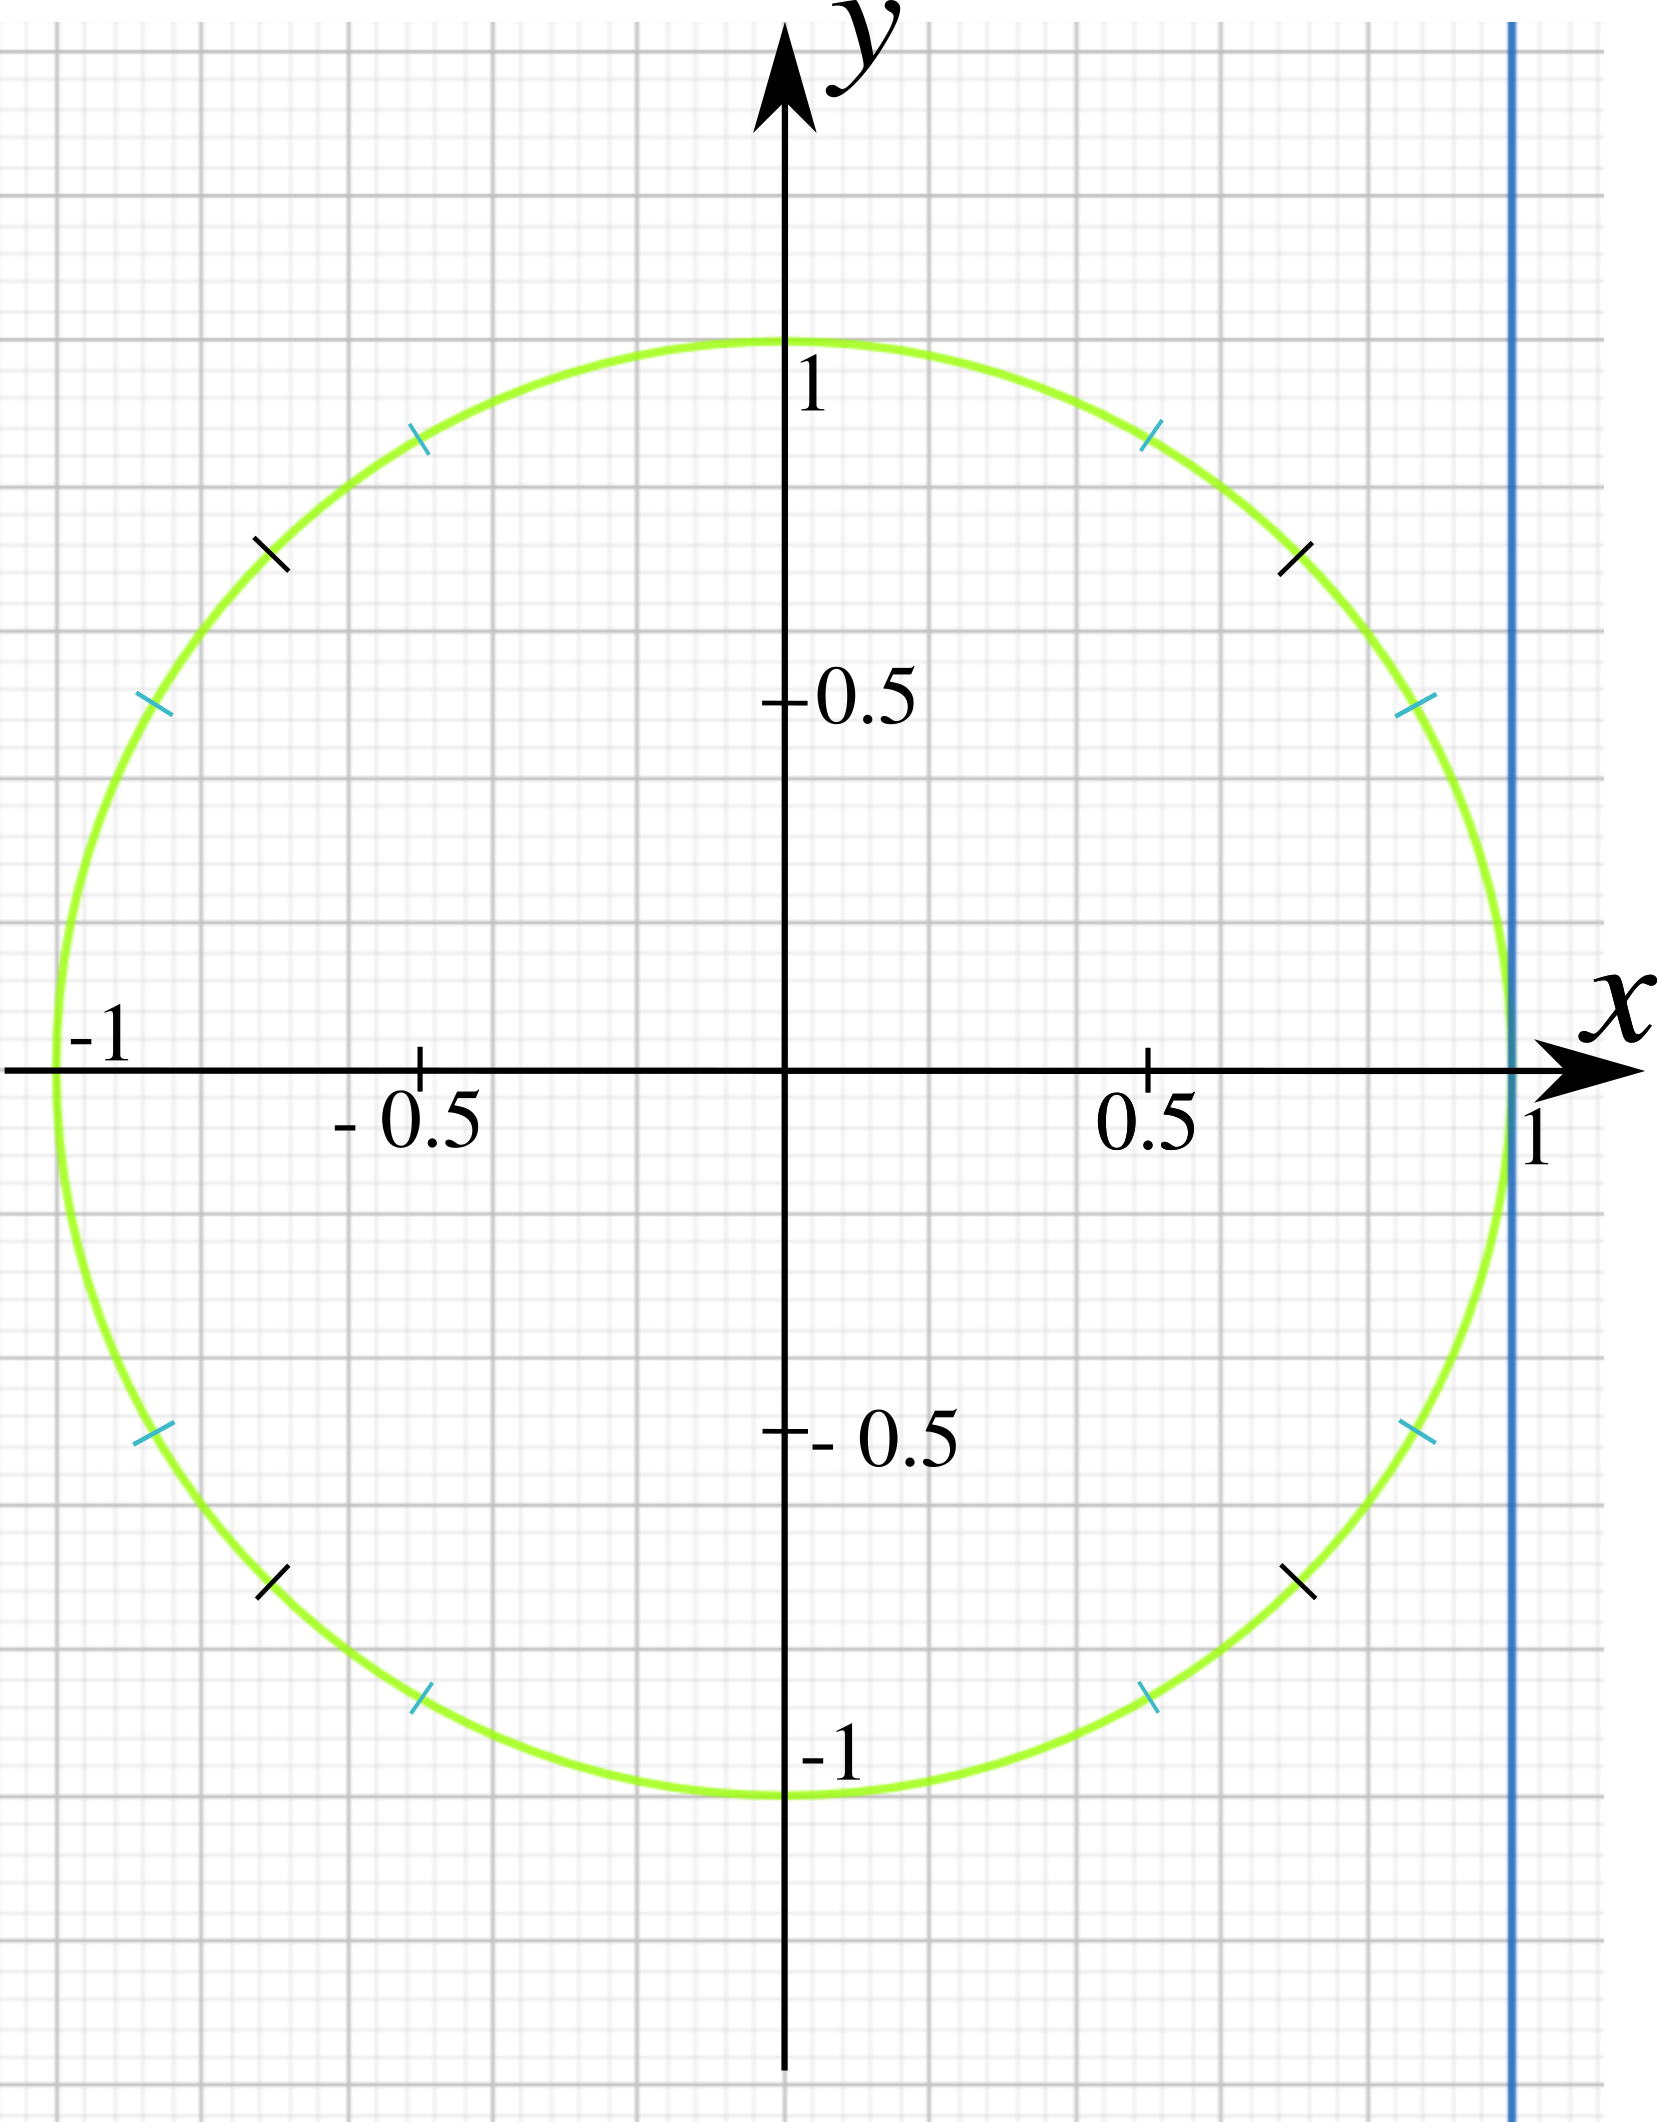
\includegraphics[width=5cm]{img/Einheitskreis304560.png}\\
\end{tabular}
}


\textbf{2. Geben Sie die Werte exakt an.} (Ohne Taschenrechner)

Tipp: Mit Hilfe eines bekannten Dreiecks.


a) $\cos(30\degre) = \LoesungsRaum{\sqrt{3}/2 \approx 0.866}$

b) $\arctan(\sqrt{3}) = \LoesungsRaum{60\degre}$

\noTRAINER{\newpage}

\noTRAINER{%
\begin{tabular}{ccc}
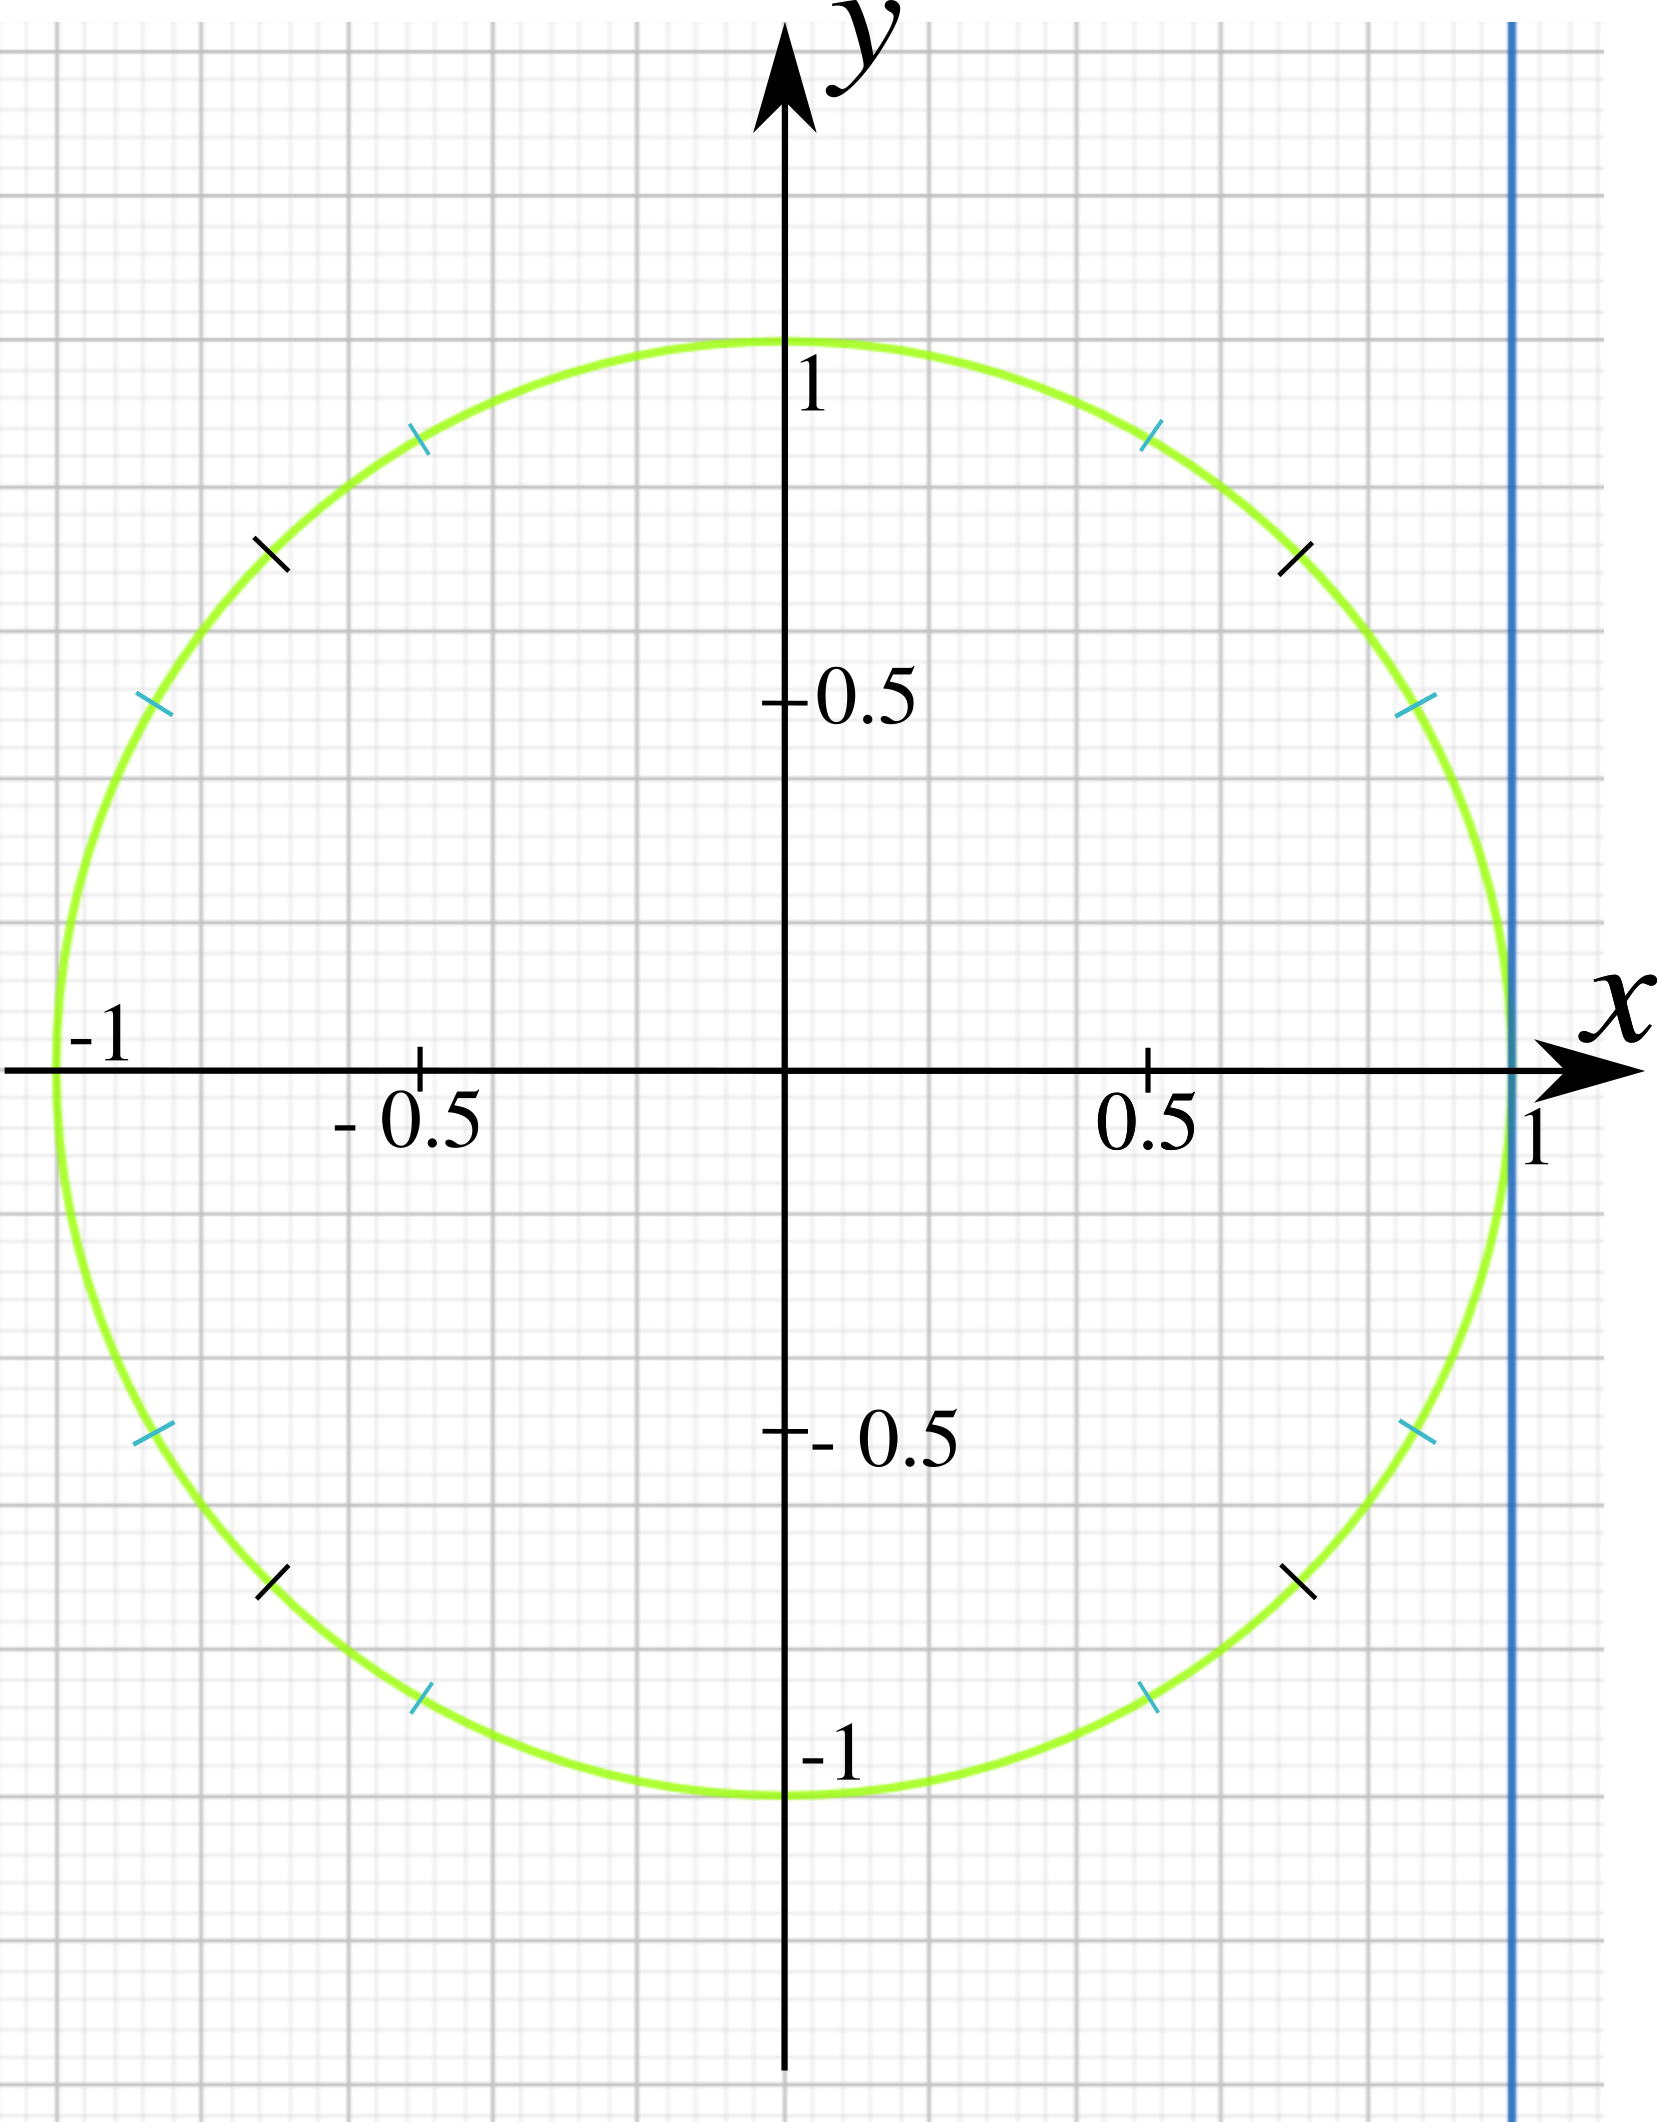
\includegraphics[width=5cm]{img/Einheitskreis304560.png} & 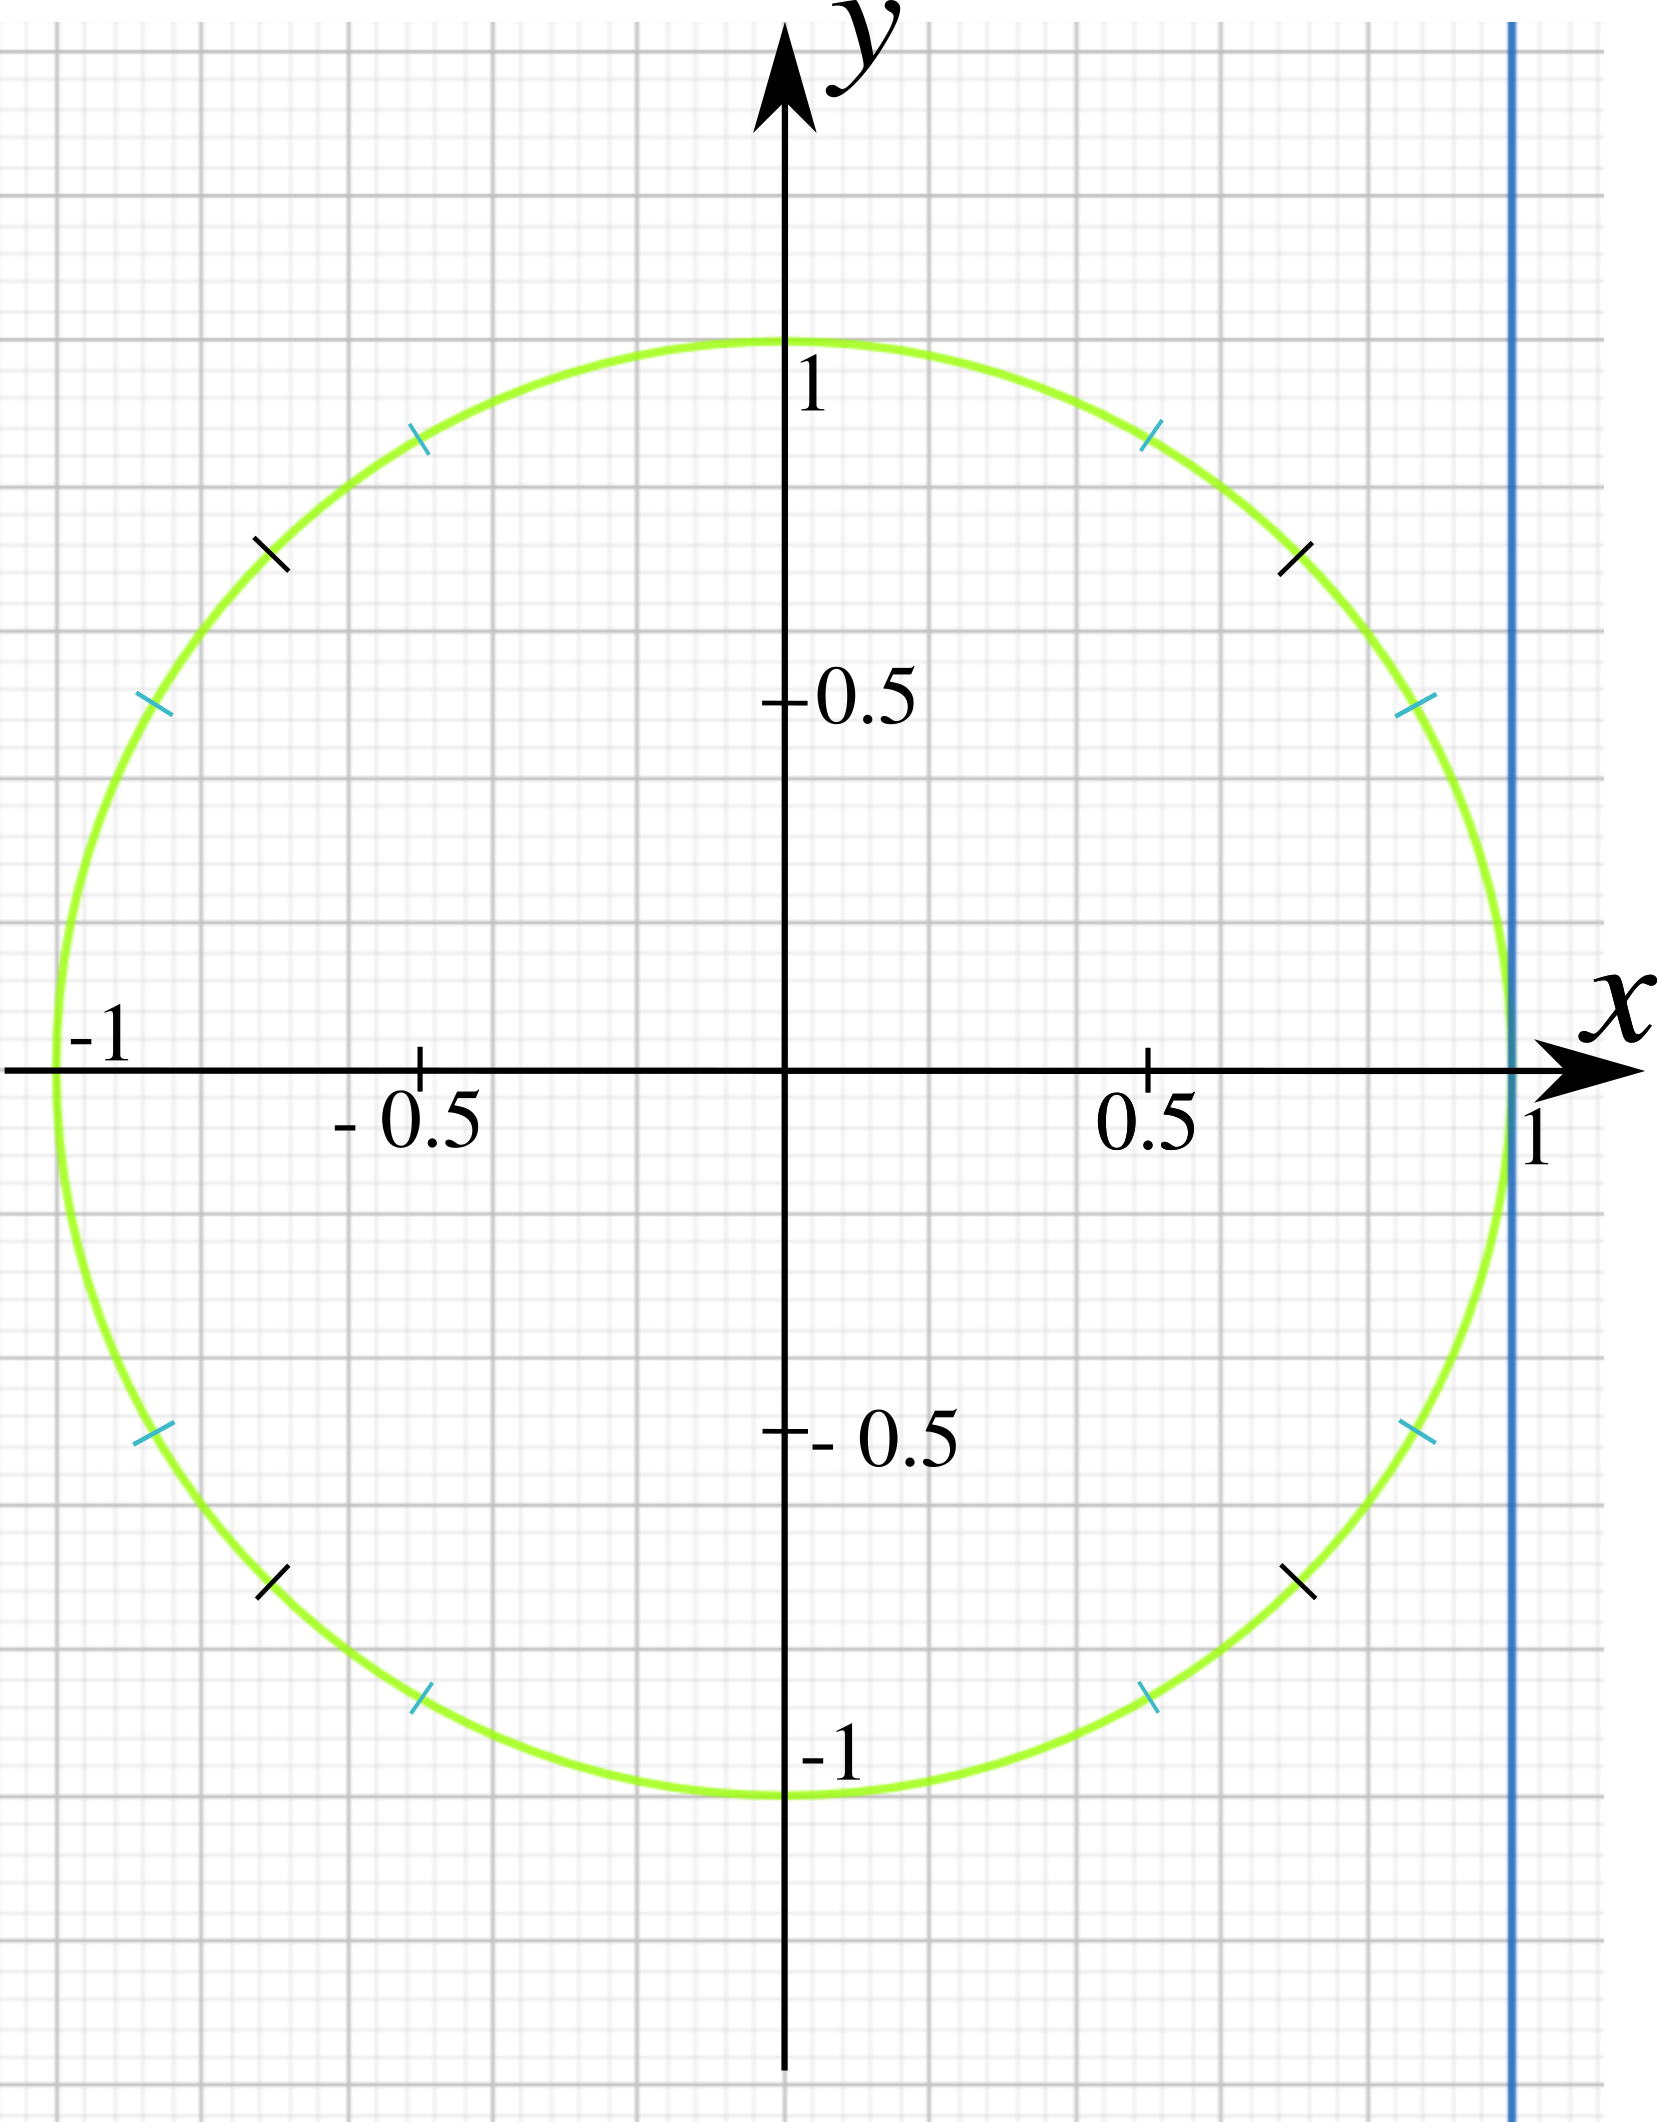
\includegraphics[width=5cm]{img/Einheitskreis304560.png} & 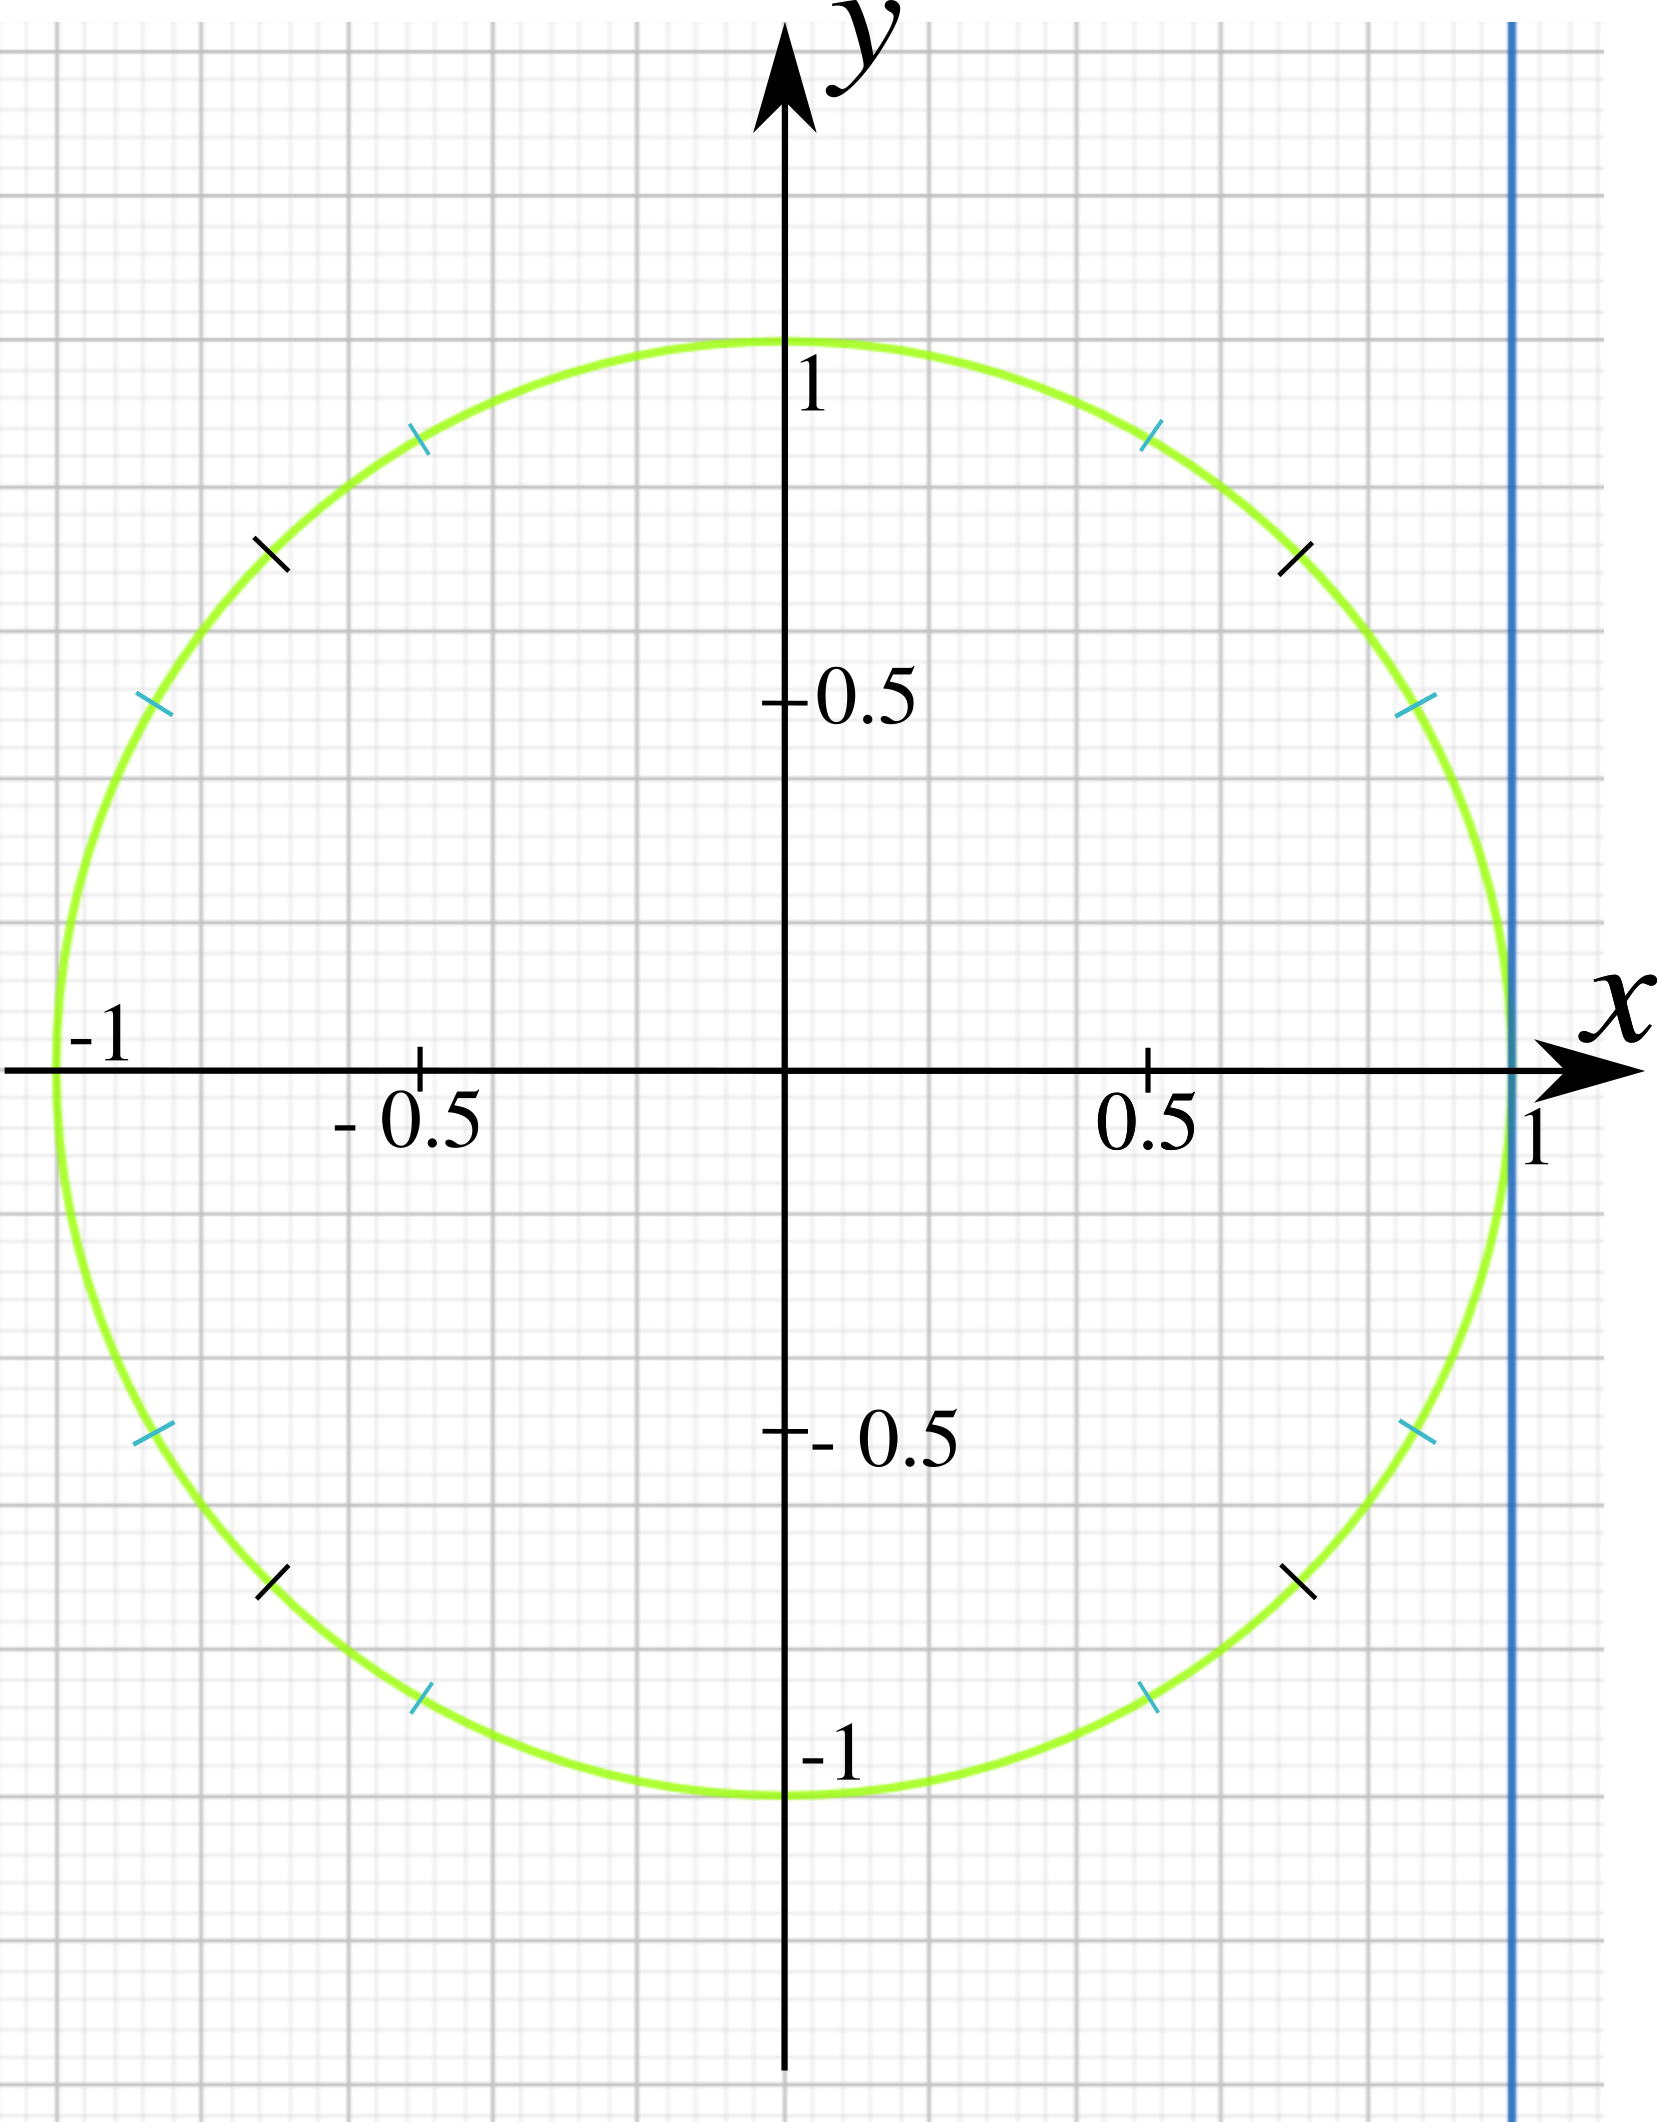
\includegraphics[width=5cm]{img/Einheitskreis304560.png}\\
\end{tabular}%
}

\textbf{3. Entscheiden Sie ob die folgenden Aussagen wahr oder falsch sind.} (Ohne Hilfe des Taschenrechners.)


a) $\cos(\alpha) = -\cos(-\alpha)$  \LoesungsRaum{falsch: Es gilt $\cos(\alpha) = \cos(-\alpha)$.}

Für $\cos(\alpha)\cdot{}\cos(\alpha)$ schreiben wir häufig auch $\cos^2(\alpha)$.

b) $\cos(\alpha^2) = \cos^2(\alpha) = \LoesungsRaum{falsch}$

c) $\cos(\alpha) = \cos(\alpha - 360\degre)$ \LoesungsRaum{Wahr. Der Einheitskreis ist zyklisch}

d) $\sin(\alpha) = -\sin(-\alpha)$ \LoesungsRaum{Wahr: An der $x$-Achse gespiegelt}


\noTRAINER{
\begin{tabular}{ccc}
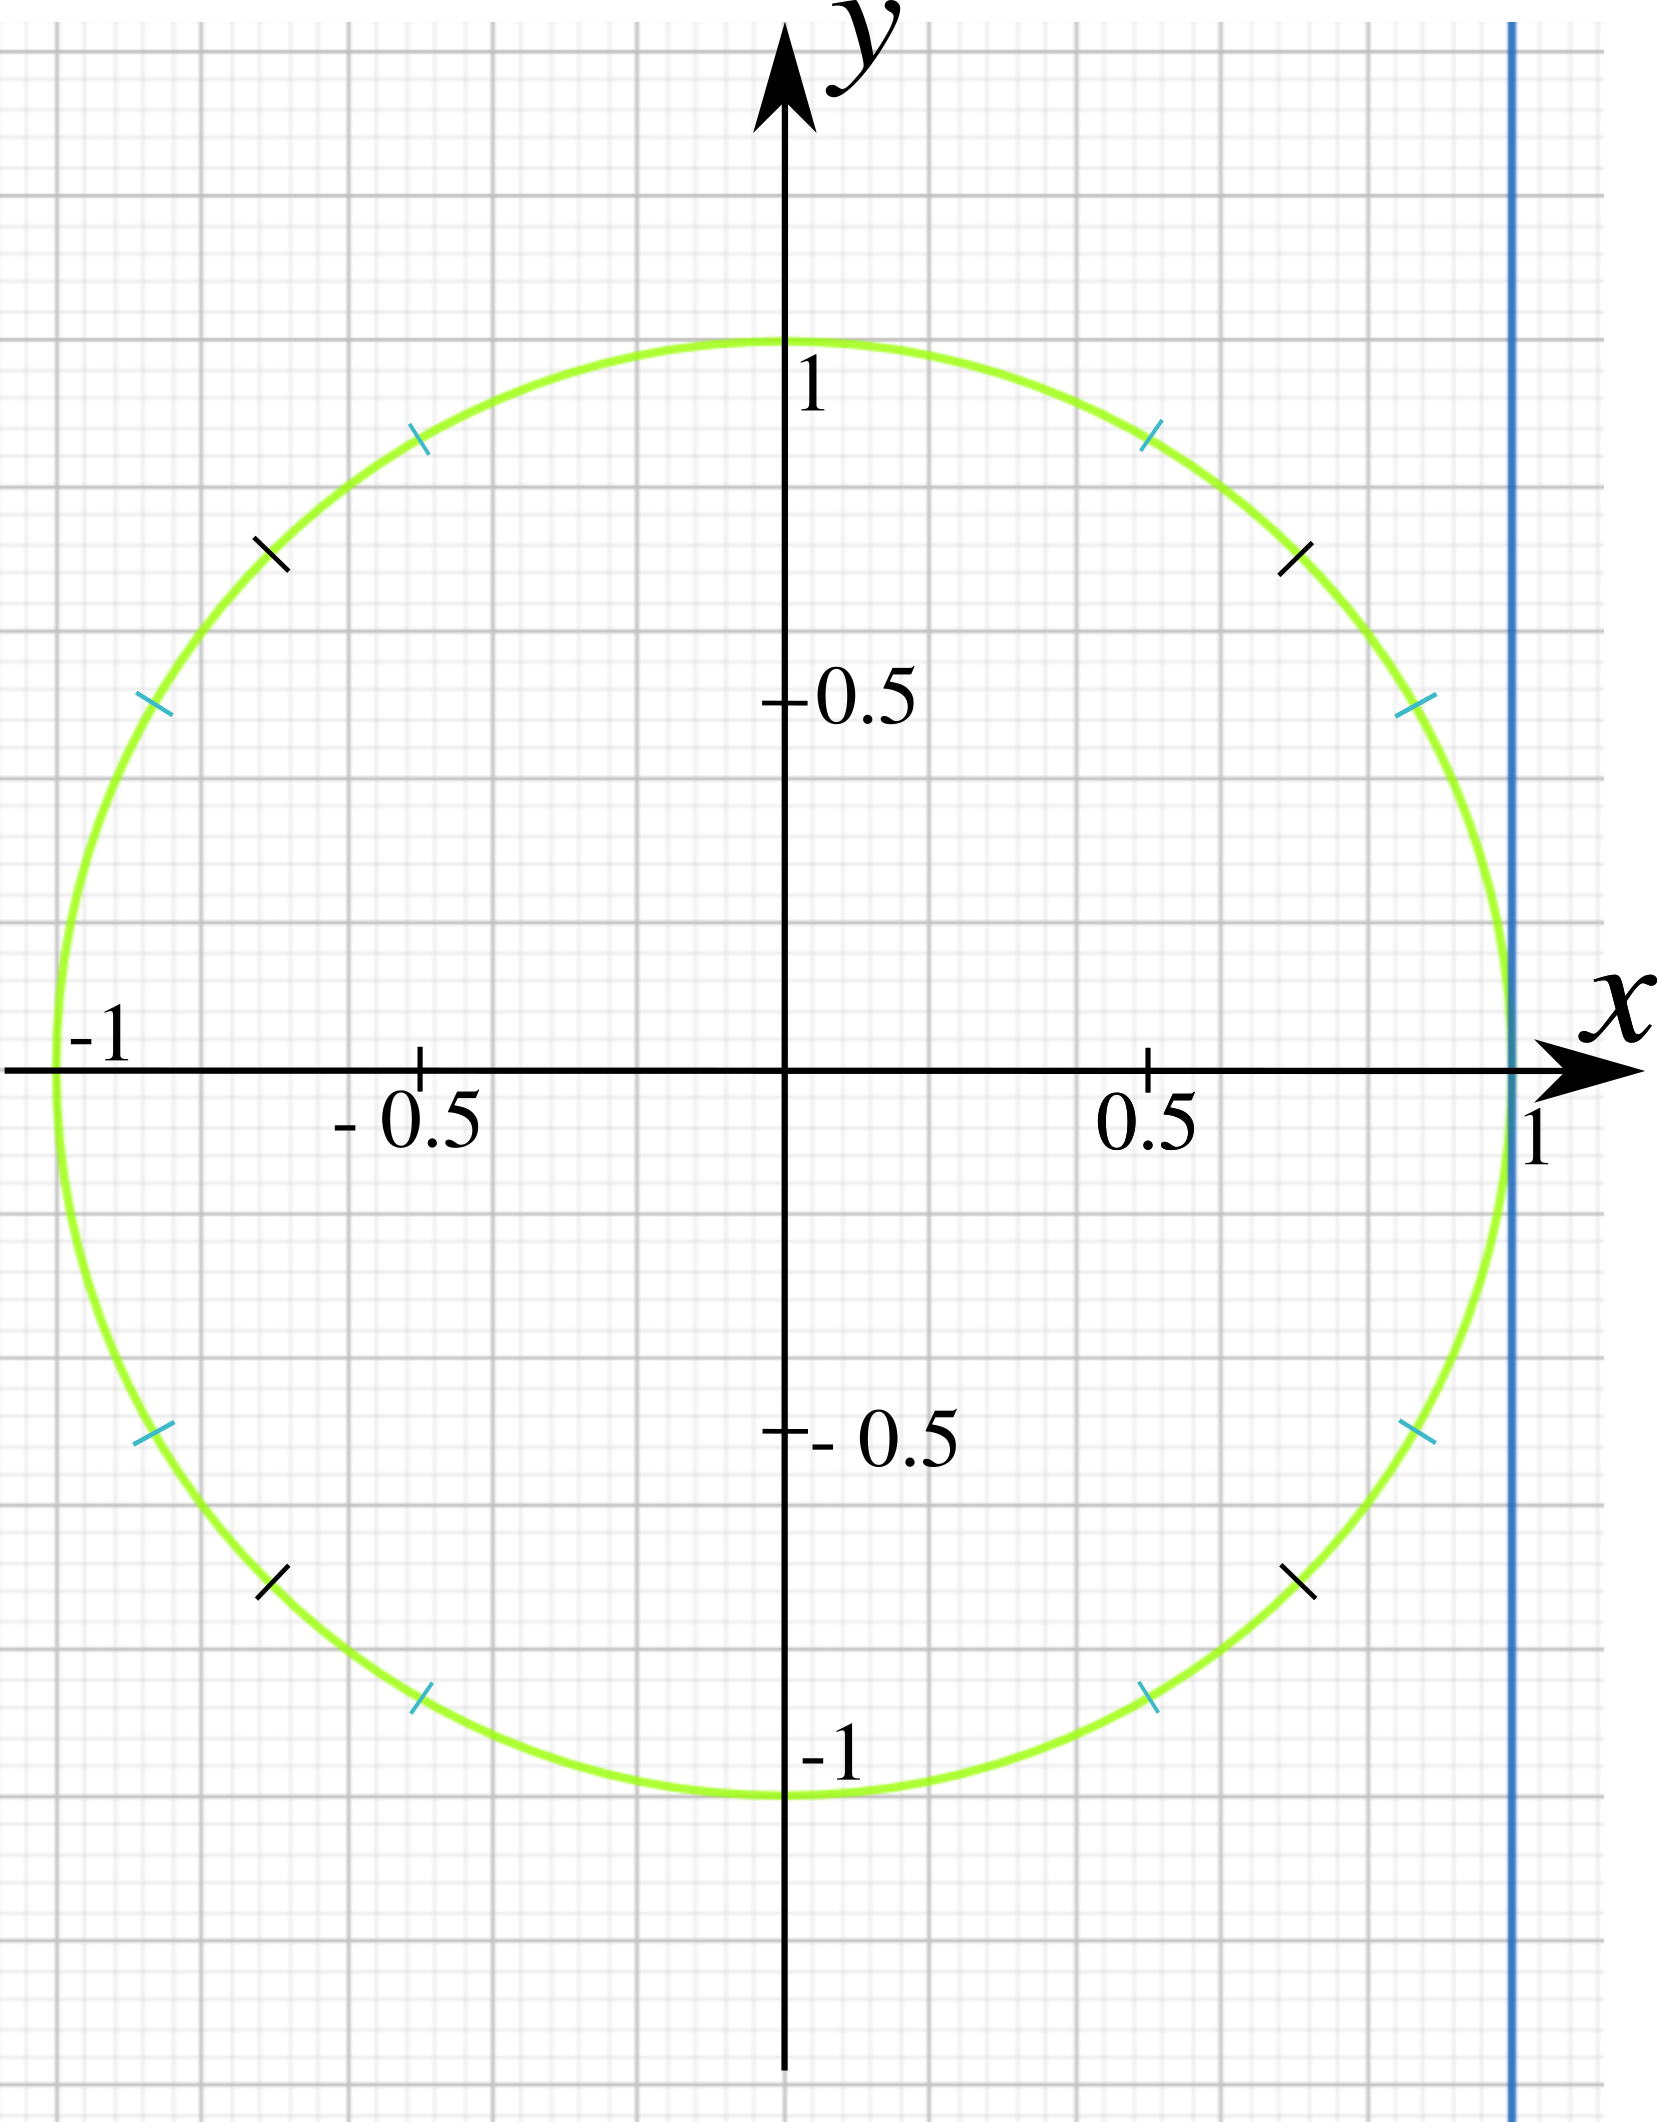
\includegraphics[width=5cm]{img/Einheitskreis304560.png} & 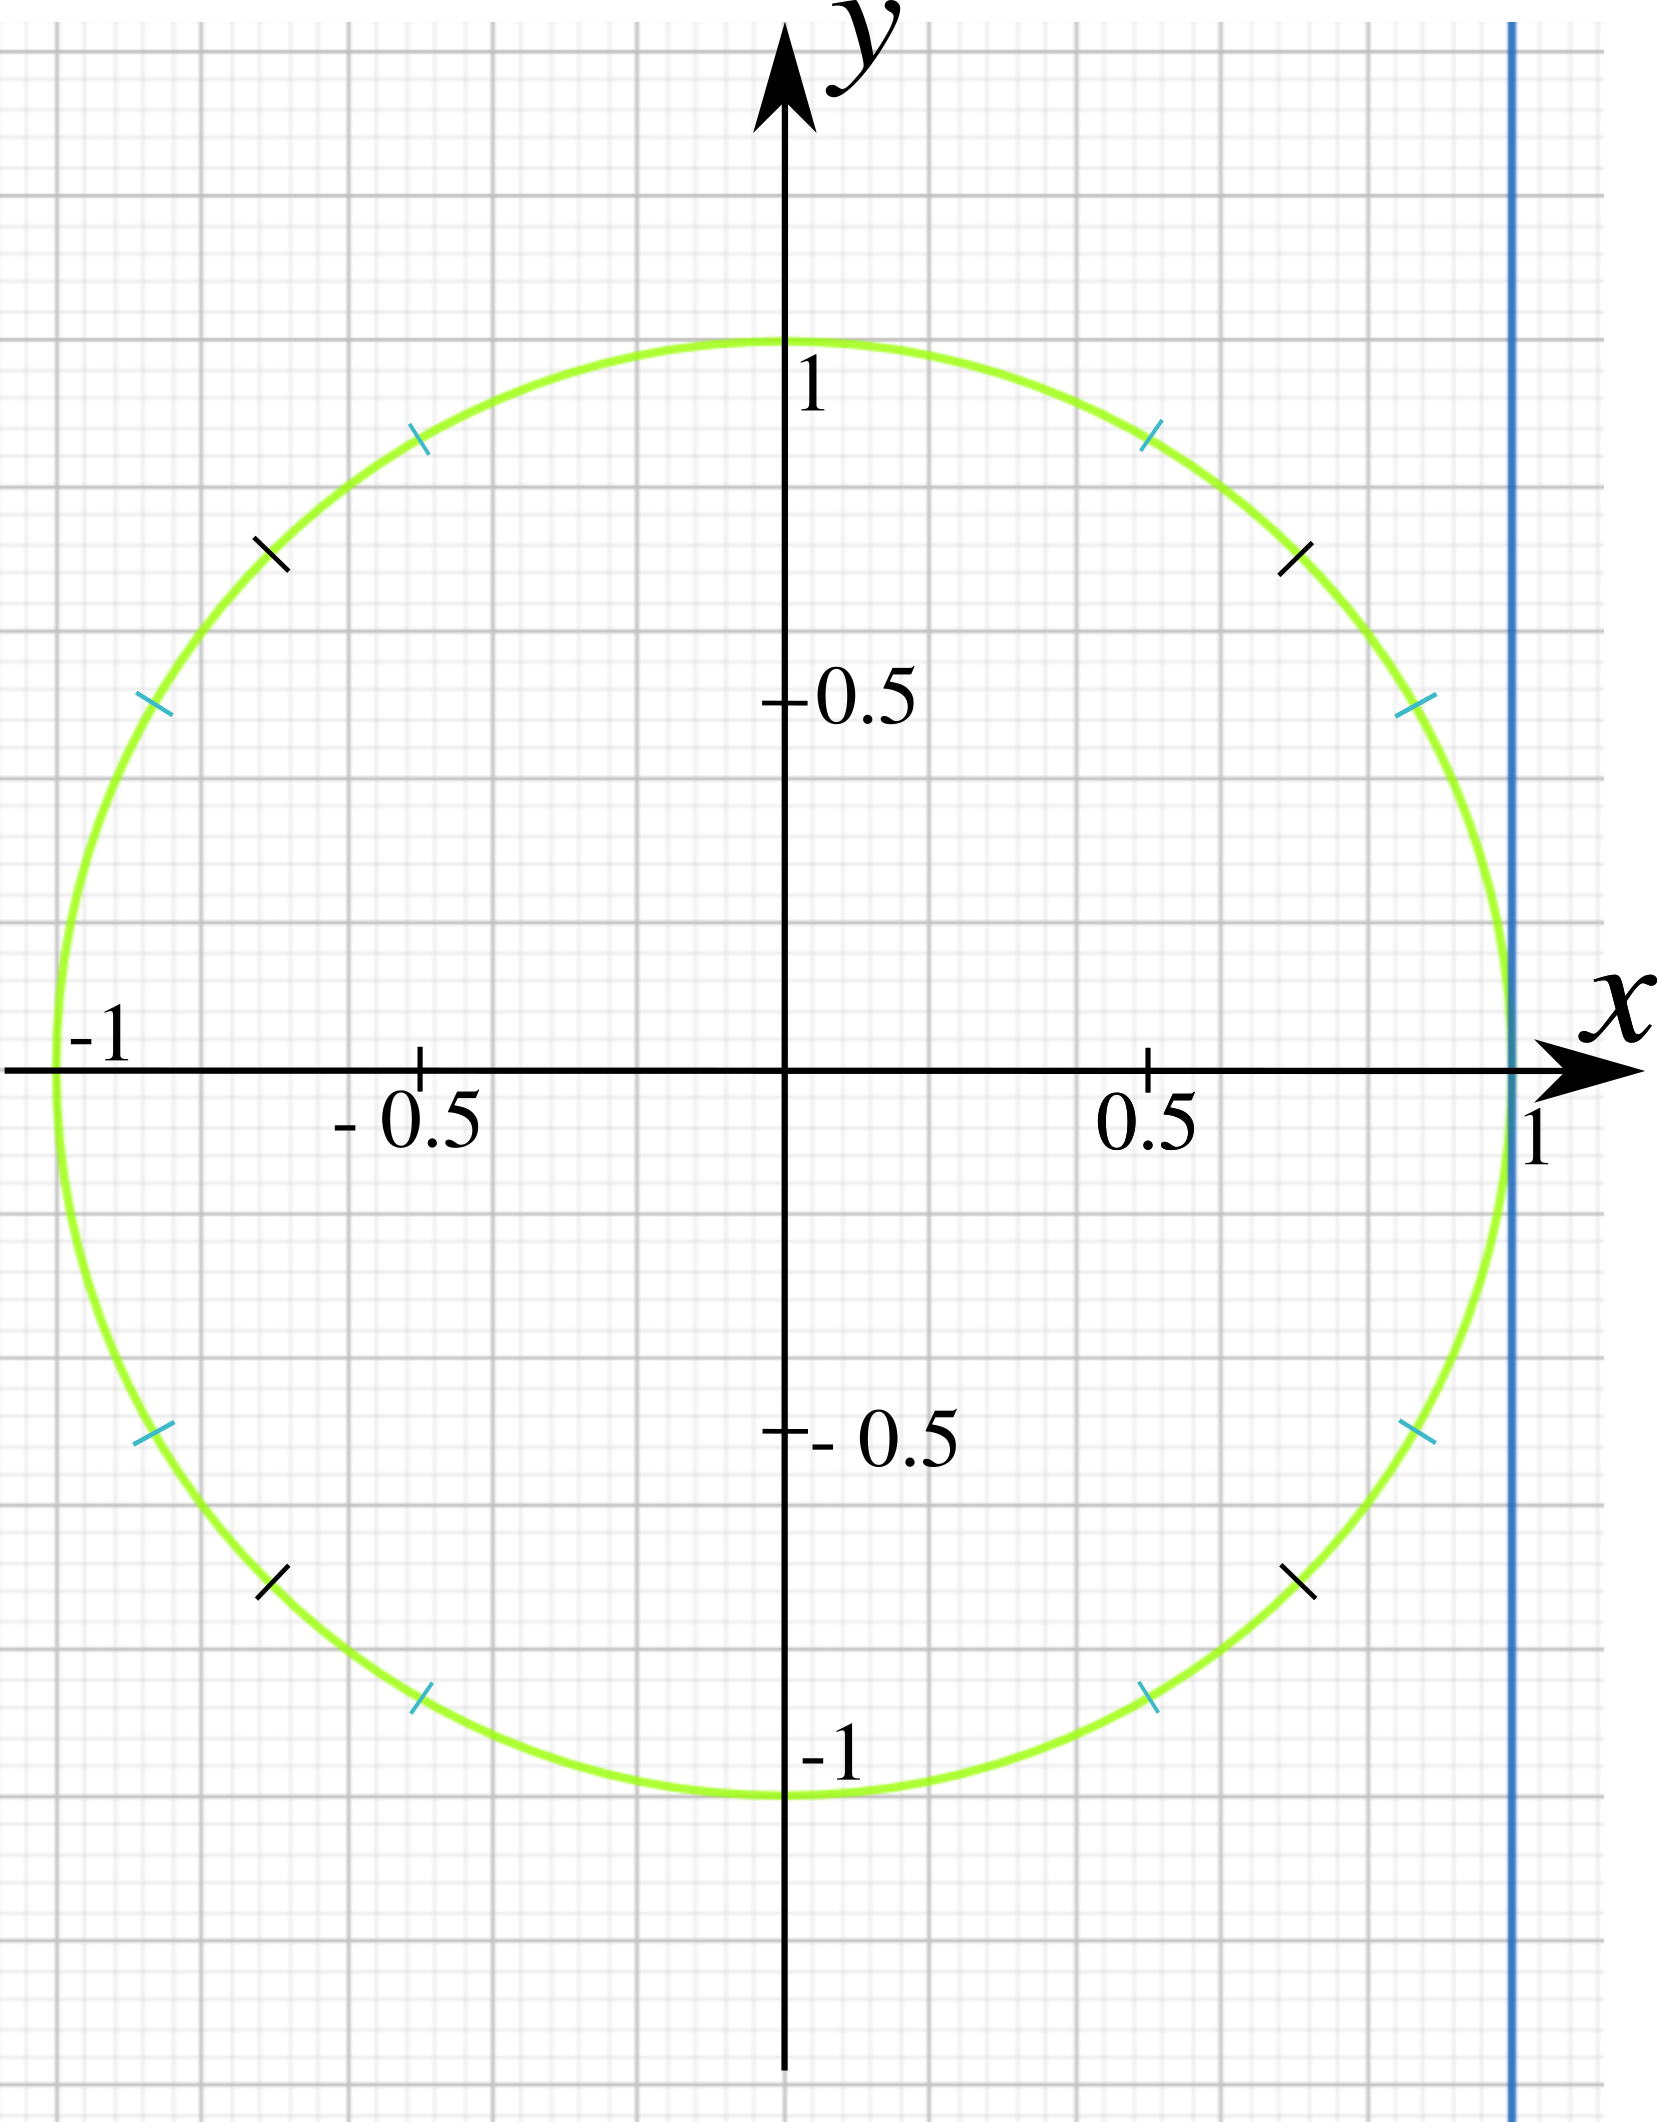
\includegraphics[width=5cm]{img/Einheitskreis304560.png} & 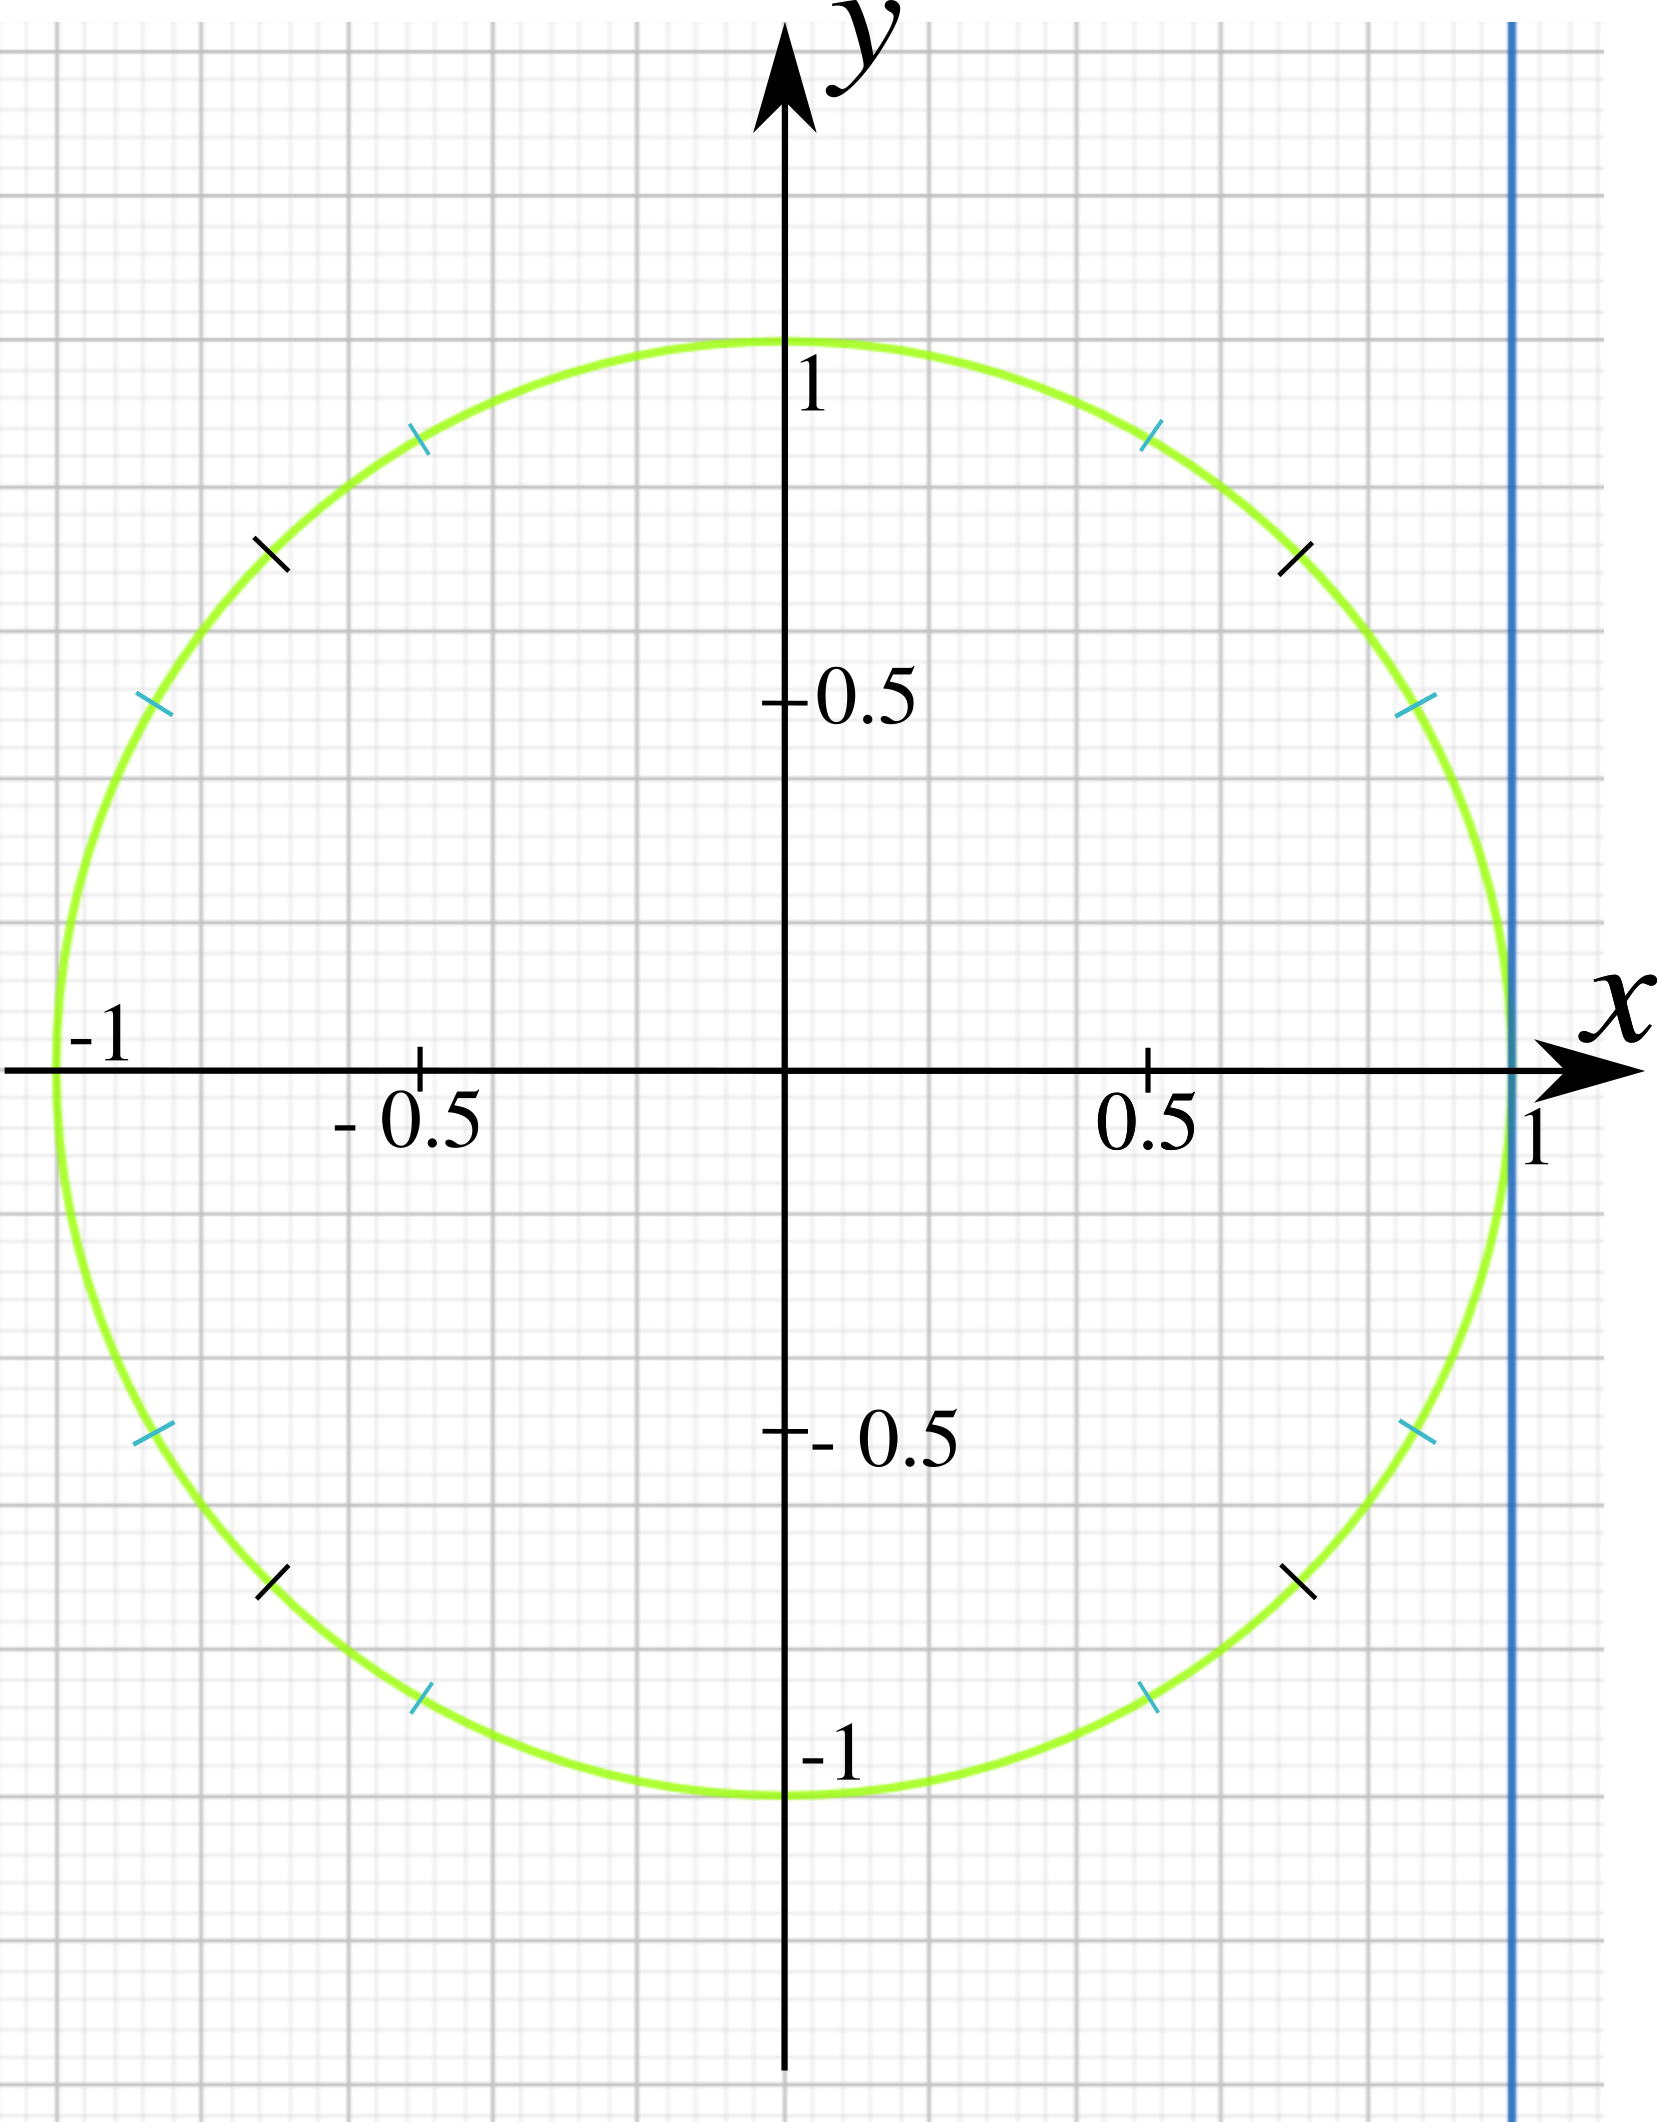
\includegraphics[width=5cm]{img/Einheitskreis304560.png}\\
\end{tabular}
}

e) $\sin(\alpha) = -\sin(\alpha - 180\degre)$ \LoesungsRaum{Wahr: Am Ursprung O gespiegelt.}

f) $\sin(\alpha) =  \sin(180\degre + \alpha )$ \LoesungsRaum{Falsch: Am Ursprung O spiegeln muss auch das Vorzeichen des sin() drehen.}
 
g) $\sin(135\degre) = \cos(135\degre)$ \LoesungsRaum{Fals: Sin ist positiv, Cos ist negativ: Die Werte sind gleich}

h) $\cos(\alpha) = \sin(\alpha + 90\degre)$ \LoesungsRaum{Wahr: Kresi um 90 Grad drehen: Phasenverschiebung.}

i) $\tan(\alpha)> 0$ für $0\degre < \alpha < 180\degre$ \LoesungsRaum{Nein, nur von 0 bis 90 (90 ausgeschossen), dann wieder von 180 bis 270}
\end{document}
  
